\documentclass[dvipsnames]{beamer}
\usepackage[utf8]{inputenc}
\usepackage{listings}
\usepackage{comment}
\usepackage{soul}
%\usepackage{ulem}
\usepackage{subfig}
\setul{}{1pt}
\usepackage[oldenum, olditem]{paralist}
%allow even smaller text
\newcommand\tinytiny{\fontsize{4pt}{3}\selectfont}

\makeatletter
\let\old@lstKV@SwitchCases\lstKV@SwitchCases
\def\lstKV@SwitchCases#1#2#3{}
\makeatother
\usepackage{lstlinebgrd}
\makeatletter
\let\lstKV@SwitchCases\old@lstKV@SwitchCases

\lst@Key{numbers}{none}{%
    \def\lst@PlaceNumber{\lst@linebgrd}%
    \lstKV@SwitchCases{#1}%
    {none:\\%
     left:\def\lst@PlaceNumber{\llap{\normalfont
                \lst@numberstyle{\thelstnumber}\kern\lst@numbersep}\lst@linebgrd}\\%
     right:\def\lst@PlaceNumber{\rlap{\normalfont
                \kern\linewidth \kern\lst@numbersep
                \lst@numberstyle{\thelstnumber}}\lst@linebgrd}%
    }{\PackageError{Listings}{Numbers #1 unknown}\@ehc}}
\makeatother


\graphicspath{{logos/}}

%disclaimer for Sandia. uncomment and the whole blob goes away @ b80c116300122
\def\sandid{SAND2020-7908 PE}

% \title{Performance Portability with Kokkos}
\title{The Kokkos Lectures}

%BAD misuse of author field
\author{Module 3: MultiDimensional Loops and Data Structures}

%\author{
%  Jeff Miles \inst{1},
%  Christian Trott \inst{1}
%}
%\institute[shortinst]{\tiny \inst{1} Sandia National Laboratories, \inst{2} Oak Ridge National Laboratory \and \inst{3} Los Alamos National Laboratory}
%\institute[shortinst]{\tiny \inst{1} Sandia National Laboratories}

\usetheme{kokkos}

\newif\ifshort
\newif\ifmedium
\newif\iffull
\newif\ifnotoverview

\newcommand{\TutorialDirectory}{\texttt{Intro-Full}}
\newcommand{\ExerciseDirectory}[1]{\texttt{Exercises/#1/}}
\newcommand{\TutorialClone}{\texttt{Kokkos/kokkos-tutorials/\TutorialDirectory}}

\definecolor{darkgreen}{rgb}{0.0, 0.5, 0.0}
\definecolor{darkred}{rgb}{0.8, 0.0, 0.0}
\definecolor{orange}{rgb}{0.8, 0.33, 0.0}
\definecolor{purple}{rgb}{0.60, 0.20, 0.80}
\colorlet{bodyColor}{blue!20}
\colorlet{patternColor}{orange!30}
\colorlet{policyColor}{green!30}

% http://tex.stackexchange.com/questions/144448/color-a-text-line-in-a-code-lstlisting
\lstnewenvironment{code}[1][]%
{
  %with txfonts: OT1/txr/m/n/10
  %with default fonts: OT1/cmr/m/n/10
  %\fontfamily{cmr}\selectfont
  %\showthe\font
   \noindent
   \minipage{\linewidth}
   %\vspace{0.5\baselineskip}
   \lstset{mathescape, escapeinside={<@}{@>},
moredelim=**[is][{\btHL[fill=patternColor]}]{@pattern}{@pattern},
moredelim=**[is][{\btHL[fill=red!30]}]{@warning}{@warning},
moredelim=**[is][{\btHL[fill=policyColor]}]{@policy}{@policy},
moredelim=**[is][{\btHL[fill=bodyColor]}]{@body}{@body},
moredelim=**[is][{\btHL[fill=red!30]}]{@warning}{@warning},
moredelim=**[is][\color{black}]{@black}{@black},
moredelim=**[is][\color{blue}]{@blue}{@blue},
moredelim=**[is][\bf]{@bold}{@bold},
moredelim=**[is][\it]{@italic}{@italic},
moredelim=**[is][\color{boldblue}\bf]{@boldblue}{@boldblue},
moredelim=**[is][\color{red}]{@red}{@red},
moredelim=**[is][\color{green}]{@green}{@green},
moredelim=**[is][\color{gray}]{@gray}{@gray},
moredelim=**[is][\color{darkgreen}]{@darkgreen}{@darkgreen},
moredelim=**[is][\color{darkred}]{@darkred}{@darkred},
moredelim=**[is][\color{orange}]{@orange}{@orange},
moredelim=**[is][\color{purple}]{@purple}{@purple},
keywords={},
#1}
}
{
  \endminipage
  %\vspace{1.0\baselineskip}
}

\makeatletter
\newif\ifATOlinebackground
\lst@Key{linebackground}{\tiny}{\def\ATOlinebackground{#1}\global\ATOlinebackgroundtrue}
\makeatother

\lstnewenvironment{shell}[1][]{%
  \global\ATOlinebackgroundfalse
  \lstset{language=sh,%
    showstringspaces=false,
    aboveskip=0pt,
    frame=none,
    numbers=none,
    belowskip=2pt,
    breaklines=true,
    #1,
    }
  %\ifATOlinebackground
  \lstset{linebackgroundcolor={
    \ATOlinebackground
  }}
  %\fi
  }{}

\lstnewenvironment{cmake}[1][]{%
  \global\ATOlinebackgroundfalse
  \lstset{language=sh,%
    showstringspaces=false,
    aboveskip=0pt,
    frame=none,
    numbers=none,
    belowskip=2pt,
    breaklines=true,
    #1,
    }
  %\ifATOlinebackground
  \lstset{linebackgroundcolor={
    \ATOlinebackground
  }}
  %\fi
  }{}

\newcommand{\inlinecode}[1]{{\lstset{basicstyle=\ttfamily,keywordstyle={},showstringspaces=false}\lstinline$#1$}}
\newcommand{\inlineshell}[1]{{\lstset{basicstyle=\ttfamily,keywordstyle={},showstringspaces=false}\lstinline$#1$}}

\setbeamercolor{block title}{fg=white, bg=SandiaLightBlue}
\setbeamercolor{block body}{bg=lightgray}
\setbeamercolor{block title alerted}{fg=white, bg=SandiaRed}
\setbeamercolor{block body alerted}{bg=lightgray}



%\usepackage[texcoord,grid,gridunit=mm,gridcolor=red!10,subgridcolor=green!10]{eso-pic}
\usepackage[absolute,overlay]{textpos}





% http://tex.stackexchange.com/questions/8851/how-can-i-highlight-some-lines-from-source-code

\usepackage{pgf, pgffor}
\usepackage{listings}
\usepackage{lstlinebgrd} % see http://www.ctan.org/pkg/lstaddons

\makeatletter
%%%%%%%%%%%%%%%%%%%%%%%%%%%%%%%%%%%%%%%%%%%%%%%%%%%%%%%%%%%%%%%%%%%%%%%%%%%%%%
%
% \btIfInRange{number}{range list}{TRUE}{FALSE}
%
% Test in int number <number> is element of a (comma separated) list of ranges
% (such as: {1,3-5,7,10-12,14}) and processes <TRUE> or <FALSE> respectively

\newcount\bt@rangea
\newcount\bt@rangeb

\newcommand\btIfInRange[2]{%
    \global\let\bt@inrange\@secondoftwo%
    \edef\bt@rangelist{#2}%
    \foreach \range in \bt@rangelist {%
        \afterassignment\bt@getrangeb%
        \bt@rangea=0\range\relax%
        \pgfmathtruncatemacro\result{ ( #1 >= \bt@rangea) && (#1 <= \bt@rangeb) }%
        \ifnum\result=1\relax%
            \breakforeach%
            \global\let\bt@inrange\@firstoftwo%
        \fi%
    }%
    \bt@inrange%
}
\newcommand\bt@getrangeb{%
    \@ifnextchar\relax%
        {\bt@rangeb=\bt@rangea}%
        {\@getrangeb}%
}
\def\@getrangeb-#1\relax{%
    \ifx\relax#1\relax%
        \bt@rangeb=100000%   \maxdimen is too large for pgfmath
    \else%
        \bt@rangeb=#1\relax%
    \fi%
}

%%%%%%%%%%%%%%%%%%%%%%%%%%%%%%%%%%%%%%%%%%%%%%%%%%%%%%%%%%%%%%%%%%%%%%%%%%%%%%
%
% \btLstHL<overlay spec>{range list}
%
% TODO BUG: \btLstHL commands can not yet be accumulated if more than one overlay spec match.
%
\newcommand<>{\btLstHL}[2]{%
  \only#3{\btIfInRange{\value{lstnumber}}{#1}{\color{#2}\def\lst@linebgrdcmd{\color@block}}{\def\lst@linebgrdcmd####1####2####3{}}}%
}%
\makeatother






% http://tex.stackexchange.com/questions/15237/highlight-text-in-code-listing-while-also-keeping-syntax-highlighting
%\usepackage[T1]{fontenc}
%\usepackage{listings,xcolor,beramono}
\usepackage{tikz}

\makeatletter
\newenvironment{btHighlight}[1][]
{\begingroup\tikzset{bt@Highlight@par/.style={#1}}\begin{lrbox}{\@tempboxa}}
{\end{lrbox}\bt@HL@box[bt@Highlight@par]{\@tempboxa}\endgroup}

\newcommand\btHL[1][]{%
  \begin{btHighlight}[#1]\bgroup\aftergroup\bt@HL@endenv%
}
\def\bt@HL@endenv{%
  \end{btHighlight}%
  \egroup
}
\newcommand{\bt@HL@box}[2][]{%
  \tikz[#1]{%
    \pgfpathrectangle{\pgfpoint{1pt}{0pt}}{\pgfpoint{\wd #2}{\ht #2}}%
    \pgfusepath{use as bounding box}%
    \node[anchor=base west, fill=orange!30,outer sep=0pt,inner xsep=1pt, inner ysep=0pt, rounded corners=3pt, minimum height=\ht\strutbox+1pt,#1]{\raisebox{1pt}{\strut}\strut\usebox{#2}};
  }%
}
\makeatother



\usetikzlibrary{calc}
\usepackage{xparse}%  For \NewDocumentCommand

% tikzmark command, for shading over items
\newcommand{\tikzmark}[1]{\tikz[overlay,remember picture] \node (#1) {};}

\makeatletter
\NewDocumentCommand{\DrawBox}{s O{}}{%
    \tikz[overlay,remember picture]{
    \IfBooleanTF{#1}{%
        \coordinate (RightPoint) at ($(left |- right)+(\linewidth-\labelsep-\labelwidth,0.0)$);
    }{%
        \coordinate (RightPoint) at (right.east);
    }%
    \draw[red,#2]
      ($(left)+(-0.2em,0.9em)$) rectangle
      ($(RightPoint)+(0.2em,-0.3em)$);}
}

\NewDocumentCommand{\DrawBoxWide}{s O{}}{%
    \tikz[overlay,remember picture]{
    \IfBooleanTF{#1}{%
        \coordinate (RightPoint) at ($(left |- right)+(\linewidth-\labelsep-\labelwidth,0.0)$);
    }{%
        \coordinate (RightPoint) at (right.east);
    }%
    \draw[red,#2]
      ($(left)+(-\labelwidth,0.9em)$) rectangle
      ($(RightPoint)+(0.2em,-0.3em)$);}
}

\NewDocumentCommand{\DrawBoxWideBlack}{s O{}}{%
    \tikz[overlay,remember picture]{
    \IfBooleanTF{#1}{%
        \coordinate (RightPoint) at ($(left |- right)+(\linewidth-\labelsep-\labelwidth,0.0)$);
    }{%
        \coordinate (RightPoint) at (right.east);
    }%
    \draw[black,#2]
      ($(left)+(-\labelwidth,0.9em)$) rectangle
      ($(RightPoint)+(0.2em,-0.3em)$);}
}
\makeatother

\usetikzlibrary{positioning}

\usetikzlibrary{shapes}

\hypersetup{
    colorlinks=true,
    linkcolor=blue,
    filecolor=magenta,
    urlcolor=cyan,
}



\shortfalse
\mediumtrue
\fulltrue
\notoverviewtrue

\begin{document}

% \begin{frame}
%   \titlepage
% \end{frame}
% 
%==============================================================================

\begin{frame}{NVIDIA's NVLABS LOGISTICS (1)}

\textbf{\large SOFTWARE FOR LAB}

\vspace{10pt}

\textbf{Remote Desktop Software:} \\
\begin{itemize}
\item {Download NoMachine now for best performance from \\
 \textbf{\ul{www.nomachine.com/download}}}
\item {Alternatively you may use a VNC client or the provided browser-based VNC option}
\end{itemize}

\vspace{10pt}

\textbf{SSH Access Software (optional):}
\begin{itemize}
\item PuTTy for Windows can be downloaded from \textbf{\ul{www.putty.org}}
\item{Alternatively you may use a provided browser-based SSH option}
\end{itemize}

\end{frame}

%==============================================================================

\begin{frame}{NVIDIA's NVLABS LOGISTICS (2)}

\textbf{\Large CONNECTION INSTRUCTIONS}
\begin{itemize}
\item {Navigate to \textbf{\ul{nvlabs.qwiklab.com}}}
\item {Login or create a new account}
\item {Select the \textbf{Instructor-Led Hands-on Labs} Class}
\item {Find the lab called \textbf{Kokkos, ...}, select it, click Select, and finally click Start}
\item {After a short wait, lab instance Connection information will be shown}
\item {Please ask Lab Assistants for help!}
\end{itemize}

\end{frame}

%==============================================================================



\begin{frame}
	\titlepage
\end{frame}

\begin{frame}{Welcome to Kokkos}

\textbf{Online Resources}:

\begin{itemize}
        \item \url{https://github.com/kokkos}:
                \begin{itemize}
                        \item Primary Kokkos GitHub Organization
                \end{itemize}
        \item \url{https://kokkos.github.io/kokkos-core-wiki}
                \begin{itemize}
			\item{Slides, recording and Q\&A for the Lectures}
                \end{itemize}
        \item \url{https://kokkos.org/kokkos-core-wiki}:
                \begin{itemize}
                        \item Wiki including API reference
                \end{itemize}
        \item \url{https://kokkosteam.slack.com}:
                \begin{itemize}
                        \item Slack channel for Kokkos.
                        \item Please join: fastest way to get your questions answered.
                        \item Can whitelist domains, or invite individual people.
                \end{itemize}
\end{itemize}

\end{frame}


\begin{frame}{Lecture Series Outline}

\begin{itemize}
        \item Module 1: Introduction, Building and Parallel Dispatch
        \item Module 2: Views and Spaces
	\item \textbf{Module 3: Data Structures + MultiDimensional Loops}
        \item Module 4: Hierarchical Parallelism
        \item Module 5: Tasking, Streams and SIMD
        \item Module 6: Internode: MPI and PGAS
        \item Module 7: Tools: Profiling, Tuning and Debugging
        \item Module 8: Kernels: Sparse and Dense Linear Algebra
        \item Module 9: Fortran inter-op
\end{itemize}
\end{frame}

\begin{frame}[fragile]{Module 1: Summary}
	\textbf{Kokkos Ecosystem}

	\textbf{Building Kokkos}

	\textbf{Data Parallelism:}

	\begin{itemize}
		\item Simple parallel loops use the \texttt{parallel\_for} pattern:
\begin{code}[linebackgroundcolor={\btLstHL<1->{3}{bodyColor}},frame=single]
@patternparallel_for@pattern("Label",@policyN@policy, [=] (int64_t i) {
  /* loop body */
});
\end{code}
\item Reductions combine contributions from loop iterations
\begin{code}[linebackgroundcolor={\btLstHL<1->{3}{bodyColor}},frame=single]
int result;
@patternparallel_reduce@pattern("Label",@policyN@policy, [=] (int64_t i, int& lres) {
   /* loop body */
    lres += /* something */
  },result);
\end{code}

\end{itemize}

	\textbf{Recording:} \url{https://bit.ly/kokkos-lecture-series-1}

\end{frame}



\begin{frame}[fragile]{Module 2: Summary}
	\textbf{Kokkos View}
	\begin{itemize}
		\item Multi Dimensional Array.
		\item Compile and Runtime Dimensions.
		\item Reference counted like a \texttt{std::shared\_ptr} to an array.
	\end{itemize}
\begin{code}[keywords={View,int}]
	Kokkos::View<int*[5]> a("A", N);
	a(3,2) = 7;
\end{code}

	\textbf{Execution Spaces}
	\begin{itemize}
		\item{Parallel operations execute in a specified \textbf{Execution Space}}
		\item{Can be controlled via template argument to \textbf{Execution Policy}}
		\item{If no Execution Space is provided use \texttt{DefaultExecutionSpace}}
	\end{itemize}
\begin{code}[keywords={parallel_for,Cuda,RangePolicy}]
// Equivalent:
parallel_for("L", N, functor);
parallel_for("L",
  RangePolicy<DefaultExecutionSpace>(0, N), functor);
\end{code}
\end{frame}

\begin{frame}[fragile]{Module 2: Summary}
	\textbf{Memory Spaces}
	\begin{itemize}
		\item Kokkos Views store data in \textbf{Memory Spaces}.
		\item Provided as template parameter.
		\item If no Memory Space is given, use  \texttt{Kokkos::DefaultExecutionSpace::memory\_space}.
		\item \texttt{deep\_copy} is used to transfer data: no hidden memory copies by Kokkos.
	\end{itemize}
\begin{code}[keywords={View,int,CudaSpace,create_mirror_view}]
	View<int*, CudaSpace> a("A", M);
	// View in host memory to load from file
	auto h_a = create_mirror_view(a);
        load_from_file(h_a);
	// Copy
	deep_copy(a,h_a);
\end{code}

\end{frame}

\begin{frame}[fragile]{Module 2: Summary}
	\textbf{Layouts}
	\begin{itemize}
		\item Kokkos Views use an index mapping to memory determined by a \textbf{Layout}.
		\item Provided as template parameter.
		\item If no \textbf{Layout} is given, derived from the execution space associated with the memory space.
		\item Defaults are good if you parallelize over left most index!
	\end{itemize}

\begin{code}[keywords={View,int,CudaSpace}]
	View<int**, LayoutLeft> a("A", N, M);
	View<int**, LayoutRight> b("B", N, M);

	parallel_for("Fill", N, KOKKOS_LAMBDA(int i) {
          for(int j = 0; j < M; j++) {
            a(i,j) = i * 1000 + j; // coalesced
	    b(i,j) = i * 1000 + j; // cached
          }
	});
\end{code}

\end{frame}

\begin{frame}[fragile]{Module 2: Summary}
	\textbf{Advanced Reductions}
	\begin{itemize}
        \item \texttt{parallel\_reduce} defaults to summation
        \item Kokkos reducers can be used to reduce over arbitrary operations
        \item Reductions over multiple values are supported
        \item Only reductions into scalar arguments are guaranteed to be synchronous
        \item Support for custom reductions
	\end{itemize}

\begin{code}[keywords={View,int,CudaSpace}]
    parallel_reduce("Join", n,
      KOKKOS_LAMBDA(int i, double& a, int& b) {
        int idx = foo();
        if(idx > b) b = idx;
        a += bar();
      }, result, Kokkos::Max<int>{my_max});
\end{code}

\end{frame}

\begin{frame}{Module 3}
  \begin{block}{MultiDimensional Loops}
    How to parallelize tightly nested loops using the MDRangePolicy?
  \end{block}

  \begin{block}{Subviews and Unmanaged Views}
    How to get slices of Views, View assignment rules and interoperating with external memory.
  \end{block}

  \begin{block}{Atomic Data Access}
    Using atomic functions. Implement an optimal scatter contribute pattern.
  \end{block}

  \begin{block}{DualView}
    Managing data synchronization without global understanding of data flow.
  \end{block}
\end{frame}

\begin{frame}[fragile]{MDRangePolicy}

  {\Huge Tightly Nested Loops with MDRangePolicy}

  \vspace{20pt}

  \textbf{Learning objectives:}
  \begin{itemize}
    \item{Demonstrate usage of the MDRangePolicy with tightly nested loops.}
    \item{Syntax - Required and optional settings}
    \item{Code demo and example}
  \end{itemize}

  \vspace{-20pt}

\end{frame}

%==========================================================================

\begin{frame}[fragile]{MDRangePolicy (0)}

  \textbf{Motivating example}: Consider the nested for loops:

%  \vspace{5pt}

  \lstset{mathescape, escapeinside={<@}{@>},
          language=C,
          keywords={}}

  \begin{lstlisting}%[linebackgroundcolor={
    %    \btLstHL{1-3}{darkred!20}
    %  }
    %]

  for ( int i = 0; i < N0; ++i )
  for ( int j = 0; j < N1; ++j )
  for ( int k = 0; k < N2; ++k )
    some_init_fcn(i, j, k);

  \end{lstlisting}

%  \vspace{-11pt}

%  \begin{itemize}
%    \item{Based on Kokkos lessons thus far, you might parallelize this as follows:}
%  \end{itemize}

  {Based on Kokkos lessons thus far, you might parallelize this as}


  \begin{lstlisting}%[linebackgroundcolor={
    %    \btLstHL{3-4}{bodyColor}
    %  }
    %]

  Kokkos::parallel_for("Label", N0,
                       KOKKOS_LAMBDA (const i) {
                         for ( int j = 0; j < N1; ++j )
                         for ( int k = 0; k < N2; ++k )
                          some_init_fcn(i, j, k);
                       }
                       );
  \end{lstlisting}

%  \begin{textblock*}{0.5\textwidth}(0.08\textwidth,0.235\textheight)
%    \rotatebox{90}{{\footnotesize {\color{darkred!80} section 1}}}
%  \end{textblock*}

%  \begin{textblock*}{0.5\textwidth}(0.08\textwidth,0.40\textheight)
%    \rotatebox{90}{{\footnotesize {\color{blue!80} section 2}}}
%  \end{textblock*}

%  \pause

  \vspace{-5pt}

  \begin{itemize}
    \item{\small{This only parallelizes along one dimension, leaving potential parallelism unexploited.}}
    \item{\small{What if Ni is too small to amortize the cost of constructing a parallel region, but Ni*Nj*Nk makes it worthwhile?}}
  \end{itemize}

%  \begin{itemize}
%    \item{Where will {\color{darkred!80}section 1} be run?  CPU?  GPU?}
%    \item{Where will {\color{blue!80}section 2} be run?  CPU?  GPU?}
%    \item{How do I \textbf{control} where code is executed?}
%  \end{itemize}

%  \pause
%  \vspace{5pt}

%  \hspace{20pt}{\Large $\Rightarrow$ \textbf{Execution spaces}}

\end{frame}

%==========================================================================

\begin{frame}[fragile]{MDRangePolicy (1)}
   \textbf{OpenMP has a solution: the collapse clause}

  \begin{code}[linebackgroundcolor={
        \btLstHL<1->{5}{bodyColor}
      },
      frame=single
    ]
#pragma @policyomp parallel@policy @patternfor@pattern @policycollapse(3)@policy
@patternfor@pattern (int64_t i = @policy0; i < N0@policy; ++i) {
  @patternfor@pattern (int64_t j = @policy0; j < N1@policy; ++j) {
    @patternfor@pattern (int64_t k = @policy0; k < N2@policy; ++k) {
      /* loop body */
    }
  }
}
  \end{code}

  \pause

Note this changed the policy by adding a `collapse` clause.

\pause

	\vspace{0.5cm}

	\textbf{With Kokkos you also change the policy:}

  \begin{code}[linebackgroundcolor={
        \btLstHL<1->{3}{bodyColor}
      },
      frame=single
    ]
@patternparallel_for@pattern("L", @policyMDRangePolicy<Rank<3>>({0,0,0},{N0,N1,N2})@policy, 
   KOKKOS_LAMBDA(int64_t i, int64_t j, int64_t k) {
     /* loop body */
});
  \end{code}

\end{frame}

\begin{frame}[fragile]{MDRangePolicy (2)}

\begin{block}{MDRangePolicy}
   MDRangePolicy can parallelize tightly nested loops of 2 to 6 dimensions.
\end{block}

	\vspace{0.5cm}

  \begin{code}[linebackgroundcolor={
        \btLstHL<1->{3}{bodyColor}
      },
      frame=single
    ]
@patternparallel_for@pattern("L", @policyMDRangePolicy<Rank<3>>({0,0,0},{N0,N1,N2})@policy, 
   KOKKOS_LAMBDA(int64_t i, int64_t j, int64_t k) {
     /* loop body */
});
  \end{code}

\begin{itemize}
   \item<2-> Specify the dimensionality of the loop with $Rank<DIM>$.
   \item<3-> As with Kokkos Views: only rectangular iteration spaces.
   \item<4-> Provide initializer lists for begin and end values.
   \item<5-> The functor/lambda takes matching number of indicies. 
\end{itemize}
\end{frame}

\begin{frame}[fragile]{MDRangePolicy (3)}
   \textbf{You can also do Reductions:}

  \begin{code}[linebackgroundcolor={
        \btLstHL<1->{5-6}{bodyColor}
      },
      frame=single
    ]
double result;
@patternparallel_reduce@pattern("Label", 
  @policyMDRangePolicy<Rank<3>>({0,0,0},{N0,N1,N2})@policy, 
  KOKKOS_LAMBDA(int i, int j, int k, double& lsum) {
     /* loop body */
  lsum += something;
}, result);
  \end{code}

\begin{itemize}
   \item<2-> The Policy doesn't change the rules for `parallel\_reduce`.
   \item<3-> Additional Thread Local Argument.
   \item<4-> Can do other reductions with reducers.
   \item<5-> Can use `View`s as reduction argument.
   \item<6-> Multiple reducers not yet implemented though.
\end{itemize}
\end{frame}

\begin{frame}[fragile]{MDRangePolicy (4)}
   In structured grid applications a \textbf{tiling} strategy is often used to help with caching.

	\begin{block}{Tiling}
		MDRangePolicy uses a tiling strategy for the iteration space.
	\end{block}

	\begin{itemize}
		\item Specified as a third initializer list.
		\item For GPUs a tile is handled by a single thread block.
			\begin{itemize}
				\item If you provide too large a tile size this will fail!
			\end{itemize}
		\item In Kokkos 3.3 we will add auto tuning for tile sizes. 
	\end{itemize}

\begin{code}[keywords={}]
double result;
parallel_reduce("Label", 
  MDRangePolicy<Rank<3>>({0,0,0},{N0,N1,N2},@policy{T0,T1,T2}@policy), 
  KOKKOS_LAMBDA(int i, int j, int k, double& lsum) {
     /* loop body */
  lsum += something;
}, result);
  \end{code}

\end{frame}


\begin{frame}[fragile]{MDRangePolicy (5)}

  Initializing a Matrix:
  
\begin{code}[keywords={LayoutLeft}]
View<double**,LayoutLeft> A("A",N0,N1);
parallel_for("Label", 
  MDRangePolicy<Rank<2>>({0,0},{N0,N1}), 
  KOKKOS_LAMBDA(int i, int j) {
    A(i,j) = 1000.0 * i + 1.0*j;
});
\end{code}

\begin{code}[keywords={LayoutRight}]
View<double**,LayoutRight> B("B",N0,N1);
parallel_for("Label", 
  MDRangePolicy<Rank<2>>({0,0},{N0,N1}), 
  KOKKOS_LAMBDA(int i, int j) {
    B(i,j) = 1000.0 * i + 1.0*j;
});
\end{code} 

\pause

	\textbf{How do I make sure that I get the right access pattern?}

\end{frame}


\begin{frame}[fragile]{MDRangePolicy (6)}
\begin{block}{Iteration Pattern}
MDRangePolicy provides compile time control over iteration patterns.
\end{block}

  \begin{lstlisting}[basicstyle=\large,gobble=4]
    Kokkos::Rank< N, IterateOuter, IterateInner >
  \end{lstlisting}

  \begin{itemize}
    \item{\small{\textbf{N: (Required)} the rank of the index space (limited from 2 to 6)}}
    \item{\small{\textbf{IterateOuter (Optional)} iteration pattern between tiles}}
    \begin{itemize}
      \item{\small{\textbf{Options:} Iterate::Left, Iterate::Right, Iterate::Default}}
    \end{itemize}
    \item{\small{\textbf{IterateInner (Optional)} iteration pattern within tiles}}
    \begin{itemize}
      \item{\small{\textbf{Options:} Iterate::Left, Iterate::Right, Iterate::Default}}
    \end{itemize}
  \end{itemize}
\end{frame}

%==========================================================================

\begin{frame}[fragile]{MDRangePolicy (7)}

  Initializing a Matrix fast:
  
\begin{code}[keywords={LayoutLeft,Iterate,Left,Right}]
View<double**,LayoutLeft> A("A",N0,N1);
parallel_for("Label", 
  MDRangePolicy<Rank<2,Iterate::Left,Iterate::Left>>(
	{0,0},{N0,N1}), 
  KOKKOS_LAMBDA(int i, int j) {
    A(i,j) = 1000.0 * i + 1.0*j;
});
\end{code}

\begin{code}[keywords={LayoutRight}]
View<double**,LayoutRight> B("B",N0,N1);
parallel_for("Label", 
  MDRangePolicy<Rank<2,Iterate::Right,Iterate::Right>>(
	{0,0},{N0,N1}), 
  KOKKOS_LAMBDA(int i, int j) {
    B(i,j) = 1000.0 * i + 1.0*j;
});
\end{code} 

\pause

	\begin{block}{Default Patterns Match}
Default iteration patterns match the default memory layouts!
	\end{block}
\end{frame}



%==========================================================================

\begin{frame}[fragile]{Exercise - mdrange: Initialize multi-dim views with MDRangePolicy}

  \textbf{Details}:
  \begin{small}
  \begin{itemize}
    \item Location: \ExerciseDirectory{mdrange/Begin}
    \item This begins with the \texttt{Solution} of 02
    \item Initialize the device Views x and y directly on the device using a parallel for and RangePolicy
    \item Initialize the device View matrix A directly on the device using a parallel for and MDRangePolicy
  \end{itemize}
  \end{small}

\begin{code}
  # Compile for CPU
  cmake -B build_openmp -DKokkos_ENABLE_OPENMP=ON
  cmake --build build_openmp
  # Run on CPU
  ./build_openmp/mdrange_exercise -S 26
  # Note the warnings, set appropriate environment variables
  # Compile for GPU
  cmake -B build_cuda -DKokkos_ENABLE_CUDA=ON
  cmake --build build_cuda
  # Run on GPU
  ./build_cuda/mdrange_exercise -S 26
\end{code}

\end{frame}

%==========================================================================

\begin{frame}[fragile]{Common Policy Arguments}

  \textbf{Template Parameters common to ALL policies.}

  \begin{itemize}
     \item \texttt{ExecutionSpace}: control where code executes
     \begin{itemize}
       \item{\small{\textbf{Options:} Serial, OpenMP, Threads, Cuda, HIP, ...}}
     \end{itemize}
     \item \texttt{Schedule$<$Options$>$}: set scheduling policy.
     \begin{itemize}
        \item{\small{\textbf{Options:} Static, Dynamic}}
     \end{itemize}

     \item \texttt{IndexType$<$Options$>$}: control internal indexing type
     \begin{itemize}
       \item{\small{\textbf{Options:} int, long, etc}}
     \end{itemize}

     \item \texttt{WorkTag}: enables multiple operators in one functor
	     \begin{code}[keywords={struct,Tag1,Tag2,void,int}]
struct Foo {
  struct Tag1{}; struct Tag2{};
  KOKKOS_FUNCTION void operator(Tag1, int i) const {...}
  KOKKOS_FUNCTION void operator(Tag2, int i) const {...}
  void run_both(int N) { 
    parallel_for(RangePolicy<Tag1>(0,N),*this);
    parallel_for(RangePolicy<Tag2>(0,N),*this);
  }
});
  \end{code}
  \end{itemize}

\end{frame}

%==========================================================================

\begin{frame}[fragile]{MDRangePolicy Section Summary}

  \textbf{MDRangePolicy}
  \begin{itemize}
    \item{allows for tightly nested loops similar to OpenMP's collapse clause.}
    \item{requires functors/lambdas with as many parameters as its rank is.}
    \item{works with \texttt{parallel\_for} and \texttt{parallel\_reduce}.}
    \item{uses a tiling strategy for the iteration space.}
    \item{provides compile time control over iteration patterns.}
  \end{itemize}

\end{frame}

%==========================================================================

\begin{frame}[fragile]{Subviews}

  {\Huge Subviews: Taking slices of Views}

  \vspace{20pt}

  \textbf{Learning objectives:}
  \begin{itemize}
    \item{Introduce Kokkos::subview---basic capabilities and syntax}
    \item{Suggested usage and practices}
    \item{View assignment rules}
  \end{itemize}

  \vspace{-20pt}

\end{frame}

%==========================================================================

\begin{frame}[fragile]{Subviews: Motivation}

  Sometimes you have to call functions on a subset of data:

  \vspace{5pt}

  \pause
  Example: call a frobenius norm on a matrix slice of a rank-3 tensor:
  \begin{code}[]
double special_norm(View<double***> tensor, int i) {

  auto matrix = ???;
  // Call a function that takes a matrix:
  return some_library::frobenius_norm(matrix);
}
    \end{code}
    \pause

    In Fortran or Matlab or Python you can get such a slice:

    \begin{code}
    tensor(i,:,:)
    \end{code}

    \pause
    Kokkos can do that too!
    \begin{block}{Subview}
     \texttt{Kokkos::subview} can be used to get a view to a subset of an existing \texttt{View}.
     \end{block}

\end{frame}


%==========================================================================

\begin{frame}[fragile]{Subviews (1)}

  \textbf{Subview description:}

  \vspace{5pt}

  \begin{itemize}
    \item{A subview is a ``slice'' of a View}
    \pause
    \begin{itemize}
      \item{The function template \texttt{Kokkos::subview()} takes a \texttt{View} and a slice for each dimension and returns a \texttt{View} of the appropriate shape.}
      \pause
      \item{The subview and original View point to the same data---no extra memory allocation nor copying}        
    \end{itemize}
    \pause
    \item{Can be constructed on host or within a kernel, since no allocation of memory occurs}
    \pause
    \item{Similar capability as provided by Matlab, Fortran, Python, etc., using ``colon'' notation}
  \end{itemize}

\end{frame}

%==========================================================================

\begin{frame}[fragile]{Subviews (2)}

  \textbf{Introductory Usage Demo:}

  \vspace{5pt}

  {Given a \texttt{View}:}

  \lstset{mathescape, escapeinside={<@}{@>},
          language=C,
          keywords={}}

  \begin{lstlisting}
    Kokkos::View<double***> v("v", N0, N1, N2);
  \end{lstlisting}
  
  \pause

  {Say we want a 2-dimensional slice at an index \texttt{i0} in the first dimension---that is, in Matlab/Fortran/Python notation:}
  \begin{lstlisting}
    slicei0 = v(i0, :, :);
  \end{lstlisting}

  \pause
  {This can be accomplished in Kokkos using a subview as follows:}
  \begin{lstlisting}
    auto sv_i0 = 
      Kokkos::subview(v, i0, Kokkos::ALL, Kokkos::ALL);

    // Just like in Python, you can do the same thing with
    // the equivalent of v(i0, 0:N1, 0:N2)
    auto sv_i0_other = 
      Kokkos::subview(v, i0, Kokkos::make_pair(0, N1),
                             Kokkos::make_pair(0, N2));
  \end{lstlisting}

\end{frame}


%==========================================================================

\begin{frame}[fragile]{Subviews (3)}

\textbf{Subview can take three types of slice arguments:}

\begin{itemize}
\item \textbf{Index}
\begin{itemize}
  \item For every index $i$ the rank of the resulting \texttt{View} is decreased by one.
  \item Must be between $0<=i<extent(dim)$
\end{itemize}
\item \textbf{Kokkos::pair}
\begin{itemize}
  \item References a half-open range of indices.
  \item The begin and end must be within the extents of the original view. 
\end{itemize}
\item \textbf{Kokkos::ALL}
\begin{itemize}
  \item References the entire extent in that dimension.
  \item Equivalent to providing \texttt{make\_pair(0,v.extent(dim))}
\end{itemize}
\end{itemize}

\end{frame}

\begin{frame}[fragile]{Subviews (4)}

  \textbf{Usage notes:}

  %\vspace{5pt}

  \begin{itemize}
    \item{Use \texttt{auto} for the type of a subview (unless you can't)}
      \pause
  \begin{itemize}
      \pause
    \item{The return type of \texttt{Kokkos::subview()} is implementation defined for performance reasons}
      \pause
    \item{You can also use \texttt{decltype(subview(/*...*/))} if you really need to spell name of the type somewhere}
  \end{itemize}
      \pause
    \item{Use \texttt{Kokkos::pair} for partial ranges if subview created within a kernel}
      \pause
    \item{Constructing subviews in inner loop code can have performance implications (for now\dots)}
      \pause
    \begin{itemize}
      \item{This will likely be far less of an issue in the future.}
      \pause
      \item{Prioritize readability and maintainability first, then make changes only if you see a performance impact.}
      \pause
    \end{itemize}
  \end{itemize}

\end{frame}

%==========================================================================

\begin{frame}[fragile]{Exercise---Subviews: Basic usage}

  \textbf{Details}:
  \begin{small}
  \begin{itemize}
    \item Location: \ExerciseDirectory{subview/Begin}
    \item This begins with the \texttt{Solution} of 04
    \item In the parallel reduce kernel, create a subview for row j of view A
    \item Use this subview when computing A(j,:)*x(:) rather than the matrix A
  \end{itemize}
  \end{small}

\begin{code}
  # Compile for CPU
  cmake -B build_openmp -DKokkos_ENABLE_OPENMP=ON
  cmake --build build_openmp
  # Run on CPU
  ./build_openmp/subview_exercise -S 26
  # Note the warnings, set appropriate environment variables
  # Compile for GPU
  cmake -B build_cuda -DKokkos_ENABLE_CUDA=ON
  cmake --build build_cuda
  # Run on GPU
  ./build_cuda/subview_exercise -S 26
\end{code}

\end{frame}

%==========================================================================

\begin{frame}[fragile]{Aside: View Assignment (1)}

  \textbf{\texttt{View::operator=()} just does the ``Right Thing''\textsuperscript{TM}}

  \vspace{5pt}

  \begin{itemize}
    \item{\texttt{View<int**> a; a = View<int*[5]>("b", 4)}}
    \pause
    {\color{darkgreen}{$=>$ Okay}}
    \pause
    \item{\texttt{View<int*[5]> a; a = View<int**>("b", 4, 5)}}\\
    \pause
    {\color{darkgreen}{$=>$ Okay, checked at runtime}}
    \pause
    \item{\texttt{View<int*[5]> a; a = View<int*[3]>("b", 4)}}\\
    \pause
    {\color{darkred}{$=>$ Compilation error}}
    \pause
    \item{\texttt{View<int*[5]> a; a = View<int**>("b", 4, 3)}}\\
    \pause
    {\color{darkred}{$=>$ Runtime error}}
    \pause
    \item{\texttt{View<int*, CudaSpace> a;}\\
    \texttt{a = View<int*, HostSpace>("b", 4)}}\\
    \pause
    {\color{darkred}{$=>$ Compilation error}}
    \item{\texttt{View<int**, LayoutLeft> a;}\\
    \texttt{a = View<int**, LayoutRight>("b", 4, 5)}}\\
    \pause
    {\color{darkred}{$=>$ Compilation error}}
  \end{itemize}

\end{frame}

%==========================================================================

\begin{frame}[fragile]{Aside: View Assignment (2)}

  \textbf{\texttt{View::operator=()} just does the ``Right Thing''\textsuperscript{TM}}

  \vspace{5pt}

  \begin{itemize}
    \item{\texttt{View<const int*> a; a = View<int*>("b", 4)}}\\
    \pause
    {\color{darkgreen}{$=>$ Okay}}
    \pause
    \item{\texttt{View<int*> a; a = View<const int*>("b", 4)}}\\
    \pause
    {\color{darkred}{$=>$ Compilation error}}
    \pause
    \item{\texttt{View<int*[5], LayoutStride> a;}\\ \texttt{a = View<int*[5], LayoutLeft>("b", 4)}}
    \pause
    {\color{darkgreen}{$=>$ Okay, converting compile-time strides into runtime strides}}
    \pause
    \item{\texttt{View<int*[5], LayoutLeft> a;}\\ \texttt{a = View<int*[5], LayoutStride>("b", 4)}}
    \pause
    {\color{yellow!50!black}{$=>$ Okay, but only if strides match layout left (checked at runtime)}}
  \end{itemize}

\end{frame}
%==========================================================================

\begin{frame}[fragile]{View Assignment: subview}

  {Given a \texttt{View}:}
  \vspace{-2pt}

  \lstset{mathescape, escapeinside={<@}{@>},
          language=C,
          keywords={}}

  \begin{lstlisting}
    Kokkos::View<int***> v("v", n0, n1, n2);
  \end{lstlisting}
  \vspace{-5pt}
  \begin{itemize}
    \item{\texttt{View<int***> a;}\\
    \texttt{a = Kokkos::subview(v, ALL, 42, ALL);}}\\
    \pause
    {\color{darkred}{$=>$ Compilation error}}
    \pause
    \item{\texttt{View<int*> a;}\\
    \texttt{a = Kokkos::subview(v, ALL, 5, 42);}}\\
    \pause
    {\color{darkgreen}{$=>$ Okay for LayoutLeft}} but {\color{darkred}{$=>$ Compilation error for LayoutRight}}
    \pause
    \item{\texttt{View<int**> a;}\\
    \texttt{a = Kokkos::subview(v, ALL, 15, ALL);}}\\
    \pause
    {\color{darkred}{$=>$ Runtime error (!)}}
    \pause
    \item{\texttt{View<int**, LayoutStride> a;}\\
    \texttt{a = Kokkos::subview(v, ALL, 15, ALL);}}\\
    \pause
    {\color{darkgreen}{$=>$ Okay}}
  \end{itemize}

\end{frame}

%==========================================================================

\begin{frame}[fragile]{Subview Summary}

  \begin{itemize}
    \item Use subviews to get a portion of a \texttt{View}. Helps with:
	    \begin{itemize}
           \item code reuse
	   \item code readability
	   \item library function compatibility
	    \end{itemize}
    \pause
    \item Kokkos supports slicing Views similar to Python/Matlab/Fortran slicing syntax 
	\begin{code}[]
auto sv = Kokkos::subview(v, 42, ALL, std::make_pair(3, 17));
	\end{code}
    \pause
    \item The return type of \texttt{subview} is complicated. Use \textbf{auto}!!
    \item {\texttt{View::operator=()} just does the ``Right Thing''\textsuperscript{TM}}
      \begin{itemize}
         \item So generally don't worry about it at first! This is advanced stuff, and more for future reference.
      \end{itemize}
  \end{itemize}

\end{frame}

\begin{frame}[fragile]{Unmanaged Views}

  {\Huge Unmanaged Views: Dealing with external memory}

  \vspace{20pt}

  \textbf{Learning objectives:}
  \begin{itemize}
    \item{Why do you need unmanaged views}
    \item{Introduce unmanaged Views - basic capabilities and syntax}
    \item{Suggested usage and practices}
  \end{itemize}

  \vspace{-20pt}

\end{frame}

\begin{frame}[fragile]{Interoperating with non-Kokkos Code}
   \textbf{Sometimes your Kokkos code can't control all allocations!}

   \begin{itemize}
	   \item Obviously best to avoid that unpleasant situation ...
   \end{itemize}

   But say you use some external function like IO classes:

\begin{code}[keywords={int,vector,string,double}]
struct MatrixReader {
  int N, M;
  std::vector<double> values;
  void read_file(std::string name) {...}
};
\end{code}

\pause
	\textbf{How can you get this to the GPU without extra allocation?}

	\pause
	\begin{block}{Unmanaged Views}
	  Views can wrap existing allocations as Unmanaged Views.
	\end{block}

\end{frame}
%==========================================================================

\begin{frame}[fragile]{Unmanaged Views (0)}

  \textbf{Unmanaged View description:}

  \vspace{5pt}
  \begin{itemize}
    \item{Normally, Views allocate memory and manage.}
    \item{Instead, Views can use externally controlled memory}
    \pause
    \item{Caveats}
    \begin{itemize}
      \item{No reference counting}
      \item{No deallocation in the constructor}
      \item{No check for the correct memory space}
    \end{itemize}
    \item{Usages}
    \begin{itemize}
      \item{Layout-punning: e.g., treat multidimensional View as one-dimensional views without copying}
      \item{Use \texttt{std::vector} or memory from CUDA library, e.g. \texttt{cuSPARSE}}
    \end{itemize}
  \end{itemize}

\end{frame}

%==========================================================================

\begin{frame}[fragile]{Unmanaged Views (1)}

  \textbf{Back to our IO example:}
  \begin{code}[keywords={int,vector,string,double}]
struct MatrixReader {
  int N, M;
  std::vector<double> values;
  void read_file(std::string name) {...}
};
  \end{code}
  
  To create an unmanaged View:
  \begin{itemize}
   \item Provide a pointer as the first constructor argument.
   \item Give all the runtime dimensions.
   \item Make sure Layout and MemorySpace match!
   \item Unmanaged Views do NOT get a label!
  \end{itemize}

  \pause
  \begin{code}[keywords={View,double,LayoutRight,HostSpace,MemoryTraits,Unmanaged}]
MatrixReader reader; reader.read_file("MM");
View<double**,LayoutRight,HostSpace>
  h_a(reader.values.data(),reader.N,reader.M);
  \end{code}

  \pause
  \textbf{How do we get this to the device?}

\end{frame}

%==========================================================================

\begin{frame}[fragile]{Unmanaged Views (2)}

  \textbf{In Module 2 we learned the Mirror Pattern}
  \begin{itemize}
    \item But the mirror pattern started with a device view!
  \end{itemize}

  \pause

  \begin{block}{Mirror in any Space}
  Kokkos::create\_mirror\_view can take a space argument for location of mirror.
  \end{block}

  \pause
  \begin{code}[keywords={}]
// Create mirror into default memory space
using space_t = DefaultExecutionSpace::memory_space;
auto a = create_mirror_view(space_t(), h_a);
// Copy values from the host to the device
deep_copy(a, h_a);
  \end{code}

  \pause
\vspace{0.5cm}
  Since the ``create mirror and then copy'' pattern is common we have a shortcut:

  \begin{code}[keywords={}]
auto a = create_mirror_view_and_copy(space_t(), h_a);
  \end{code}


\end{frame}

%==========================================================================

\begin{frame}[fragile]{Scratch Allocations}
  Using pre-allocated scratch memory for temporary data structures is common to:
  \begin{itemize}
     \item Eliminate costly allocation/deallocation operations
     \item Reduce total memory footprint.
  \end{itemize}
\pause
  \begin{block}{Unmanaged Views of Scratch Allocations}
	  Unmanaged Views can be used to get arrays of different shapes backed by the same memory.
  \end{block}
   
  \begin{code}[keywords={void,View,double}]
void* scratch = kokkos_malloc<>("Scratch", scratch_size);
View<double**> a_scr(scratch, N,M);
View<int*> b_scr(scratch,K);
  \end{code}

\pause
	How much memory do you need for a \texttt{View}?

  \begin{code}[keywords={int,View,double}]
int scratch_size = View<double**>::required_allocation_size(N,M);
  \end{code}

\end{frame}

%==========================================================================

\begin{frame}[fragile]{Unmanaged Views Summary}

\vspace{-10pt}

  \begin{itemize}
    \item{Unmanaged Views wrap existing allocations} 
    \begin{itemize}
       \item{No ref-counting}
       \item{No deallocation after losing scope}
       \item{No memory space checks}
    \end{itemize}
    \pause
    \item{Unmanaged view is created with pointer and runtime dimensions }  
    \pause
  \begin{code}[keywords={}]
void* ptr = kokkos_malloc<>("Alloc", alloc_size);
View<double**> h_a((double*)ptr,N,M);
  \end{code}
  \pause
    \item {Unmanaged view uses}
    \begin{itemize}
    \item {Access externally controlled memory }
    \item {Access temporary scratch memory}
    \item {Layout pruning - view underlying data using different layout}
    \end{itemize} 
  \end{itemize}

\end{frame}

\begin{frame}[fragile]

  \vspace{-10pt}

  {\Huge Thread safety and \\ atomic operations}

  \vspace{10pt}

  \textbf{Learning objectives:}
  \begin{itemize}
    \item{Understand that coordination techniques for low-count CPU threading are not scalable.}
    \item{Understand how atomics can parallelize the \textbf{scatter-add} pattern.}
    \item{Gain \textbf{performance intuition} for atomics on the CPU and GPU, for different data types and contention rates.}
    %\item{Understand a common thread-scalable \textbf{array-filling} algorithm.}
  \end{itemize}

  \vspace{-20pt}

\end{frame}

%==========================================================================

\begin{frame}[fragile]{Examples: Histogram}

 \begin{tikzpicture}[remember picture, overlay]
    \node [shift={(-6.4cm,1.10cm)}]  at (current page.south east)
      {%
      \begin{tikzpicture}[remember picture, overlay]
        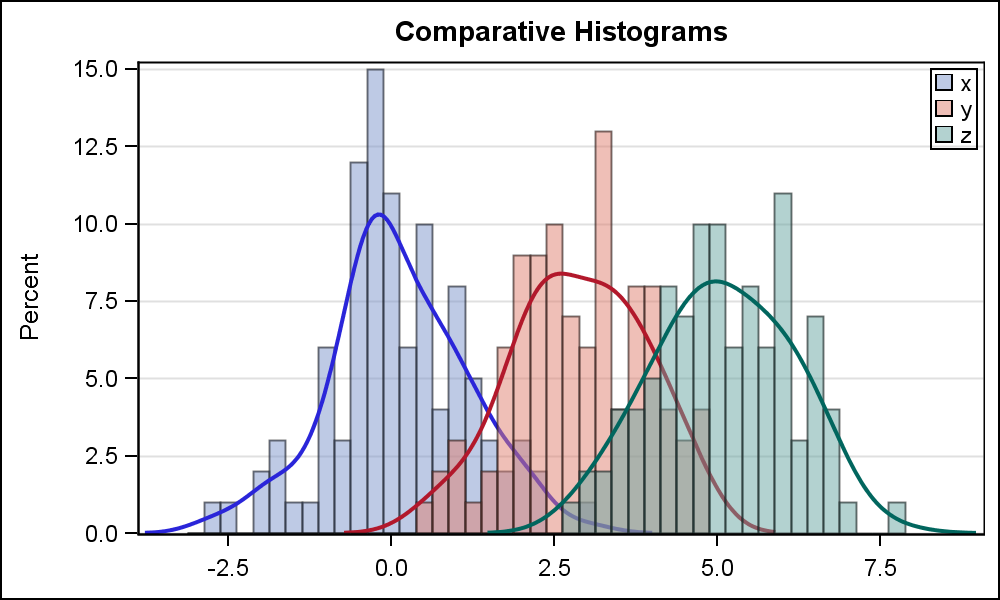
\includegraphics[width=0.50\textwidth]{figures/Histograma}
      \end{tikzpicture}
      };
  \end{tikzpicture}

  \begin{textblock*}{0.30\textwidth}(0.60\textwidth,0.91\textheight)
    \begin{tiny}
    http://www.farmaceuticas.com.br/tag/graficos/
    \end{tiny}
  \end{textblock*}

  \textbf{\ul{Histogram kernel:}}
  \begin{code}[linebackgroundcolor={
      },
      keywords={}, frame=single
    ]
parallel_for(N, KOKKOS_LAMBDA(const size_t index) {
    const Something value = ...;
    const size_t bucketIndex = computeBucketIndex(value);
    ++_histogram(bucketIndex);
  });
  \end{code}

  \pause

  {\color{red} \textbf{Problem}:} Multiple threads may try to write to the same location.

  \vspace{10pt}
  \pause

  \textbf{Solution strategies}:
  \begin{itemize}
    \item {Locks: not feasible on GPU}
    \item {Thread-private copies:\\ not thread-scalable}
    \item {Atomics}
  \end{itemize}

  \vspace{20pt}

\end{frame}

%==========================================================================

\begin{frame}[fragile]{Atomics}

  \ul{\textbf{Atomics}: the portable and thread-scalable solution}

  \begin{code}[linebackgroundcolor={
      },
      keywords={}, frame=single
    ]
parallel_for(N, KOKKOS_LAMBDA(const size_t index) {
    const Something value = ...;
    const int bucketIndex = computeBucketIndex(value);
    Kokkos::atomic_add(&_histogram(bucketIndex), 1);
  });
  \end{code}

  \pause
  \vspace{0pt}

  \begin{itemize}[<+->]
    \item {Atomics are the \textbf{only scalable} solution to thread safety.}
    \item {Locks are \textbf{not portable}.}
    \item {Data replication is \textbf{not thread scalable}.}
  \end{itemize}

  \vspace{0pt}

\end{frame}

%==========================================================================

\begin{frame}[fragile]{Performance of atomics (0)}

  \ul{\textbf{How expensive are atomics?}}

  \vspace{10pt}

  Thought experiment: scalar integration

  \begin{code}[linebackgroundcolor={
      },
      keywords={}
    ]
operator()(const unsigned int intervalIndex,
           double & valueToUpdate) const {
  double contribution = function(...);
  valueToUpdate += contribution;
}
  \end{code}

  \pause
  \vspace{10pt}
  Idea: what if we instead do this with \texttt{parallel\_for} and atomics?

  \begin{code}[linebackgroundcolor={
      },
      keywords={}
    ]
@grayoperator()(const unsigned int intervalIndex) const {
  const double contribution = function(...);@gray
  @boldKokkos::atomic_add@bold(&globalSum, contribution);
@gray}@gray
  \end{code}

  \vspace{0pt}
  How much of a performance penalty is incurred?

\end{frame}

%==========================================================================

\begin{frame}[fragile]{Performance of atomics (1)}

  \ul{\textbf{Two costs:}} (independent) {\color{blue}work} and {\color{darkred}coordination}.

  \vspace{-5pt}

  \begin{code}[linebackgroundcolor={
        \btLstHL<1->{4}{blue!20}
      },
      keywords={}
    ]
@warningparallel_reduce@warning(numberOfIntervals,
  KOKKOS_LAMBDA (const unsigned int intervalIndex,
                 double & valueToUpdate) {
    valueToUpdate += function(...);
  }, totalIntegral);
  \end{code}

  \vspace{10pt}
  \pause

  \ul{\textbf{Experimental setup}}

  \begin{code}[linebackgroundcolor={
      },
      frame=single,
      keywords={}
    ]
@grayoperator()(const unsigned int index) const {@gray
  Kokkos::atomic_add(&globalSums[index % atomicStride], 1);
@gray}@gray
  \end{code}

  \vspace{-5pt}

  \begin{itemize}
    \item{This is the most extreme case: {\color{darkred}all coordination} and {\color{darkred}no work}.}

    \item{Contention is captured by the \texttt{atomicStride}. \\
          \hspace{20pt}\texttt{atomicStride} $\rightarrow$ 1 \hspace{16pt}$\Rightarrow$ Scalar integration ({\color{darkred}bad}) \\
          \hspace{20pt}\texttt{atomicStride} $\rightarrow$ large $\Rightarrow$ Independent ({\color{darkgreen}good})
     }
  \end{itemize}

  \vspace{-15pt}

\end{frame}

%==========================================================================

\begin{frame}[fragile]{Performance of atomics (2)}

  \ul{\textbf{Atomics performance:} 1 million adds, \textbf{no} work per kernel}

  \vspace{0pt}

  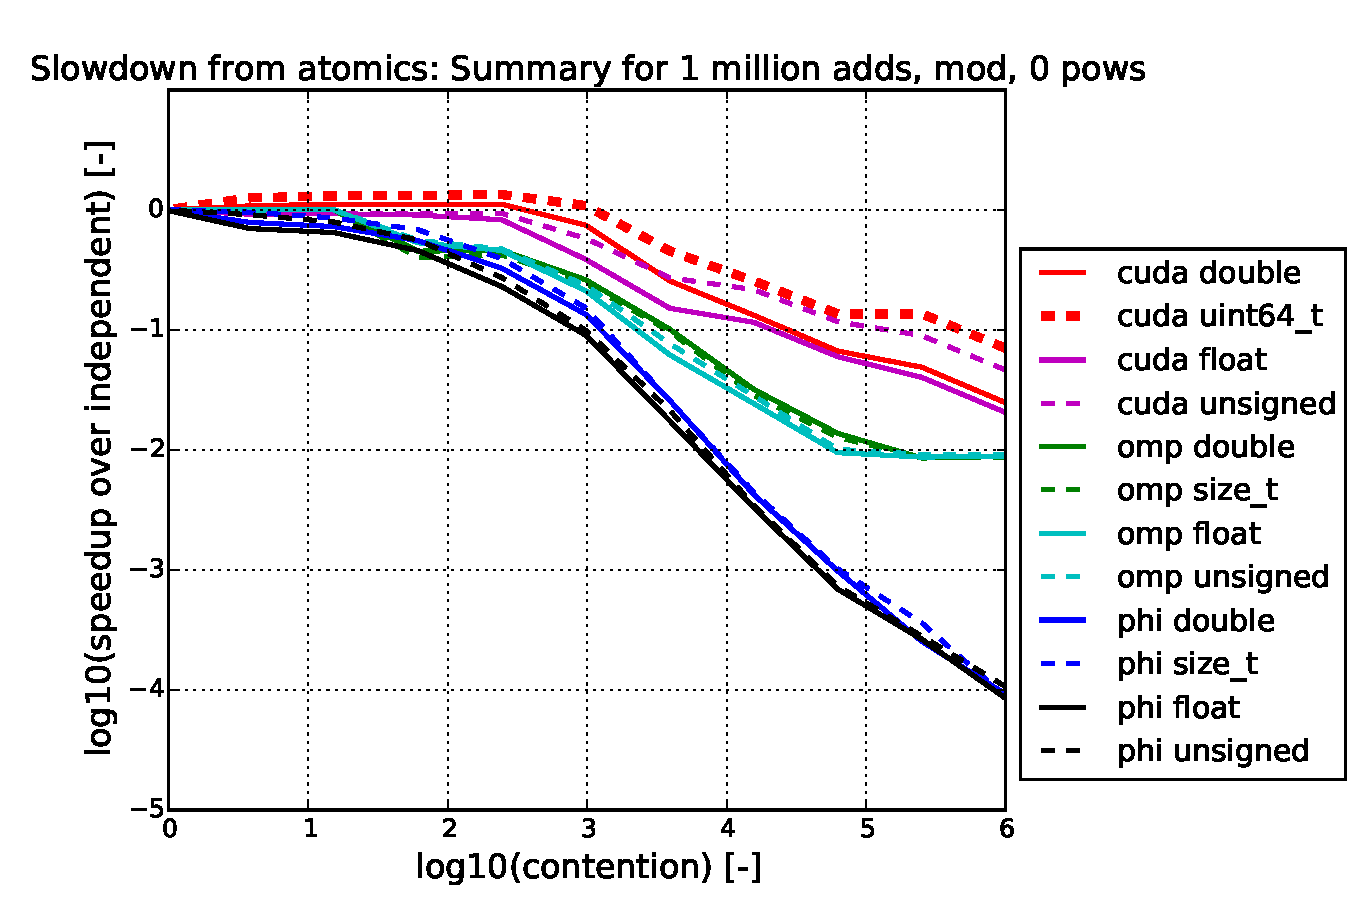
\includegraphics[width=1.00\textwidth]{figures/AtomicAddTest_slowdown_summary_mod_00pows.pdf}

  \begin{textblock*}{0.50\textwidth}(0.10\textwidth,0.45\textheight)
    \rotatebox{90}{Note: \textbf{log scale}}
  \end{textblock*}

  \pause

  \begin{textblock*}{0.70\textwidth}(0.23\textwidth,0.285\textheight)
    \only<2>{\textbf{Low(?) penalty for low contention}}
  \end{textblock*}

  \begin{tikzpicture}[remember picture, overlay]
    \node [shift={(2.40cm,6.05cm)}]  at (current page.south west)
      {%
      \begin{tikzpicture}[remember picture, overlay]
        \draw<2->[blue,ultra thick] (0.0,0.0) rectangle (2.00cm, 0.45cm);
      \end{tikzpicture}
      };
  \end{tikzpicture}


  \begin{textblock*}{0.70\textwidth}(0.35\textwidth,0.74\textheight)
    \only<2>{\textbf{High penalty for \\ high contention}}
  \end{textblock*}

  \begin{tikzpicture}[remember picture, overlay]
    \node [shift={(6.75cm,1.80cm)}]  at (current page.south west)
      {%
      \begin{tikzpicture}[remember picture, overlay]
        \draw<2->[red,ultra thick] (0.0,0.0) rectangle (2.25cm, 4.00cm);
      \end{tikzpicture}
      };
  \end{tikzpicture}
\end{frame}
\setcounter{subfigure}{0}% Reset subfigure counter

%==========================================================================

\begin{frame}[fragile]{Performance of atomics (3)}

  \ul{\textbf{Atomics performance:} 1 million adds, \textbf{some} work per kernel}

  \vspace{0pt}

  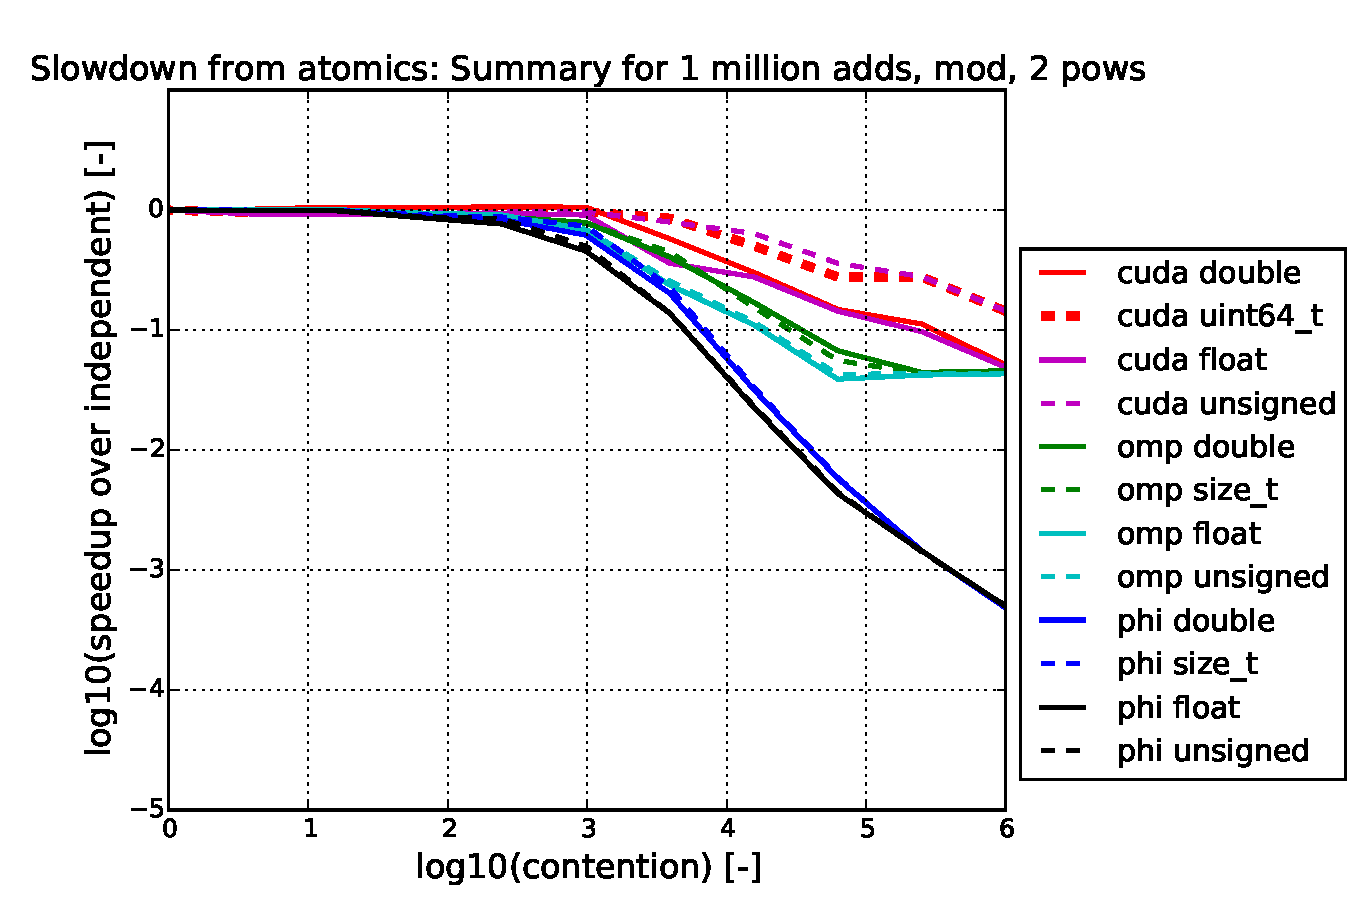
\includegraphics[width=1.00\textwidth]{figures/AtomicAddTest_slowdown_summary_mod_02pows.pdf}

  \begin{textblock*}{0.50\textwidth}(0.10\textwidth,0.45\textheight)
    \rotatebox{90}{Note: \textbf{log scale}}
  \end{textblock*}

  \begin{textblock*}{0.70\textwidth}(0.23\textwidth,0.285\textheight)
    \textbf{No penalty for low contention}
  \end{textblock*}

  \begin{tikzpicture}[remember picture, overlay]
    \node [shift={(2.40cm,5.90cm)}]  at (current page.south west)
      {%
      \begin{tikzpicture}[remember picture, overlay]
        \draw[blue,ultra thick] (0.0,0.0) rectangle (2.75cm, 0.52cm);
      \end{tikzpicture}
      };
  \end{tikzpicture}


  \begin{textblock*}{0.70\textwidth}(0.35\textwidth,0.74\textheight)
    \textbf{High penalty for \\ high contention}
  \end{textblock*}

  \begin{tikzpicture}[remember picture, overlay]
    \node [shift={(6.75cm,1.80cm)}]  at (current page.south west)
      {%
      \begin{tikzpicture}[remember picture, overlay]
        \draw[red,ultra thick] (0.0,0.0) rectangle (2.25cm, 4.00cm);
      \end{tikzpicture}
      };
  \end{tikzpicture}
\end{frame}
\setcounter{subfigure}{0}% Reset subfigure counter

%==========================================================================

\begin{frame}[fragile]{Performance of atomics (4)}

  \ul{\textbf{Atomics performance:} 1 million adds, \textbf{lots of} work per kernel}

  \vspace{0pt}

  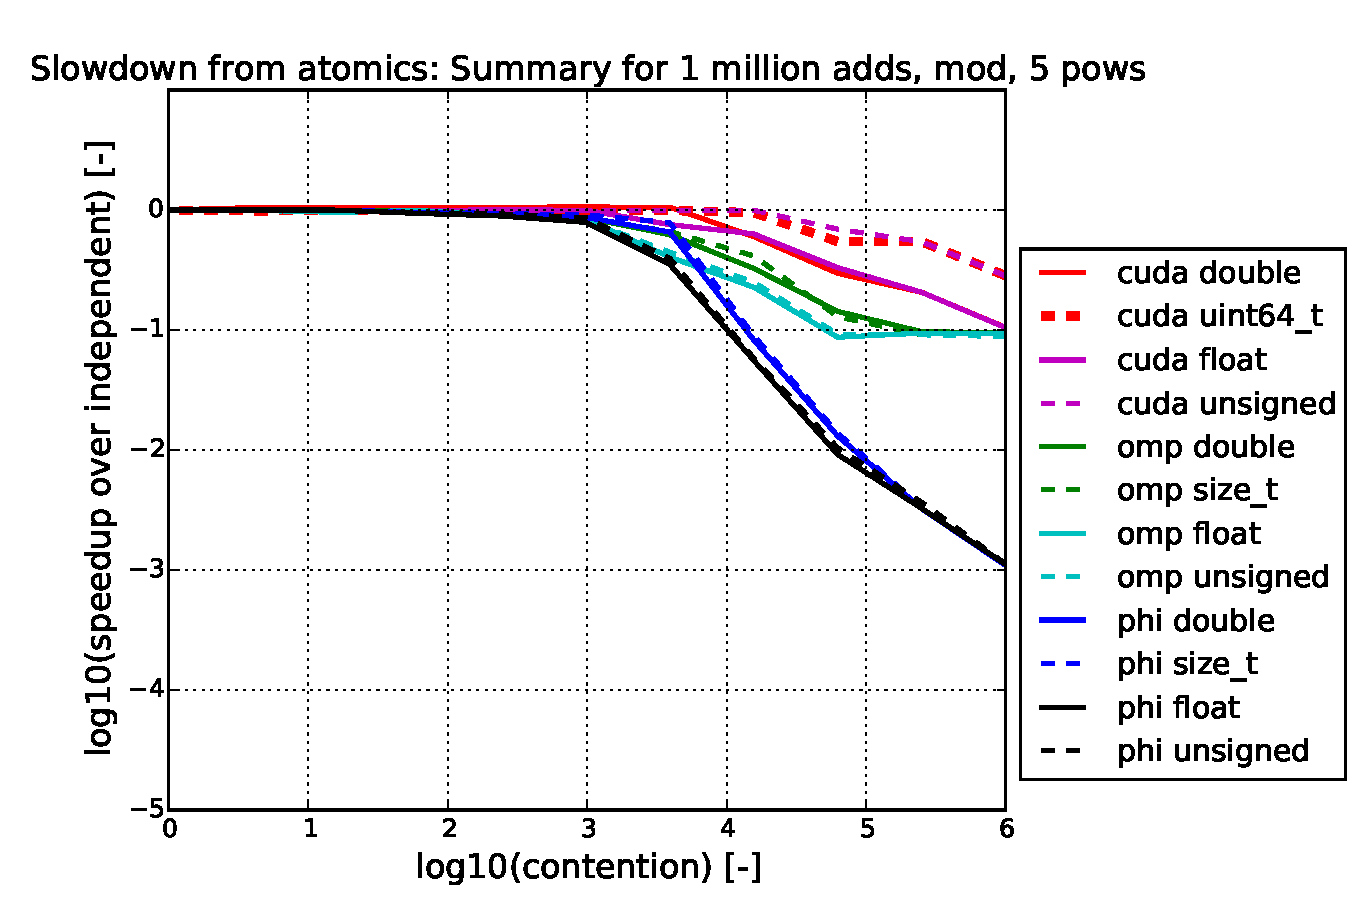
\includegraphics[width=1.00\textwidth]{figures/AtomicAddTest_slowdown_summary_mod_05pows.pdf}

  \begin{textblock*}{0.50\textwidth}(0.10\textwidth,0.45\textheight)
    \rotatebox{90}{Note: \textbf{log scale}}
  \end{textblock*}

  \begin{textblock*}{0.70\textwidth}(0.23\textwidth,0.285\textheight)
    \textbf{No penalty for low contention}
  \end{textblock*}

  \begin{tikzpicture}[remember picture, overlay]
    \node [shift={(2.40cm,5.90cm)}]  at (current page.south west)
      {%
      \begin{tikzpicture}[remember picture, overlay]
        \draw[blue,ultra thick] (0.0,0.0) rectangle (3.50cm, 0.52cm);
      \end{tikzpicture}
      };
  \end{tikzpicture}


  \begin{textblock*}{0.70\textwidth}(0.35\textwidth,0.74\textheight)
    \textbf{High penalty for \\ high contention}
  \end{textblock*}

  \begin{tikzpicture}[remember picture, overlay]
    \node [shift={(6.75cm,1.80cm)}]  at (current page.south west)
      {%
      \begin{tikzpicture}[remember picture, overlay]
        \draw[red,ultra thick] (0.0,0.0) rectangle (2.25cm, 4.00cm);
      \end{tikzpicture}
      };
  \end{tikzpicture}
\end{frame}
\setcounter{subfigure}{0}% Reset subfigure counter

%==========================================================================

\begin{frame}[fragile]{Advanced features}

\textbf{\ul{Atomics on arbitrary types}:}

\begin{itemize}
\item Atomic operations work if the corresponding operator exists,
  \hspace{50pt}i.e., \texttt{atomic\_add} works on any data type with ``+''.
\item {Atomic exchange works on any data type.}
\end{itemize}
\vspace{-10pt}
  \begin{code}[linebackgroundcolor={
      },
      keywords={}
    ]
// Assign *dest to val, return former value of *dest
template<typename T>
T atomic_exchange(T * dest, T val);
// If *dest == comp then assign *dest to val
// Return true if succeeds.
template<typename T>
bool atomic_compare_exchange_strong(T * dest, T comp, T val);
\end{code}

\end{frame}

%==========================================================================

\begin{frame}[fragile]{Memory traits}

  \textbf{\ul{Slight detour: \texttt{View} memory traits}:}

  \begin{itemize}
    \item Beyond a \texttt{Layout} and \texttt{Space}, \texttt{Views} can have memory traits.
    \item Memory traits either provide \textbf{convenience} or allow for certain \textbf{hardware-specific optimizations} to be performed.
  \end{itemize}

  Example: If all accesses to a \texttt{View} will be atomic, use the \texttt{Atomic} memory trait:

  \vspace{-2pt}
  \begin{code}[keywords={}]
    View<double**, Layout, Space,
         @boldMemoryTraits<Atomic> @bold> forces(...);
  \end{code}

  \vspace{5pt}
  \pause

  Many memory traits exist or are experimental, including \texttt{Atomic}, \texttt{Unmanaged}, \texttt{Restrict}, and \texttt{RandomAccess}.

  \vspace{-15pt}

\end{frame}

%==========================================================================

\begin{frame}[fragile]{RandomAccess memory trait}

  \textbf{\ul{Example: \texttt{RandomAccess} memory trait}:}

  \vspace{3pt}

  On \textbf{GPUs}, there is a special pathway for fast \textbf{read-only}, \textbf{random} access, originally designed for textures.

  \vspace{5pt}
  \pause

  In the early days you had to access this via \textbf{CUDA}:
  \vspace{5pt}
  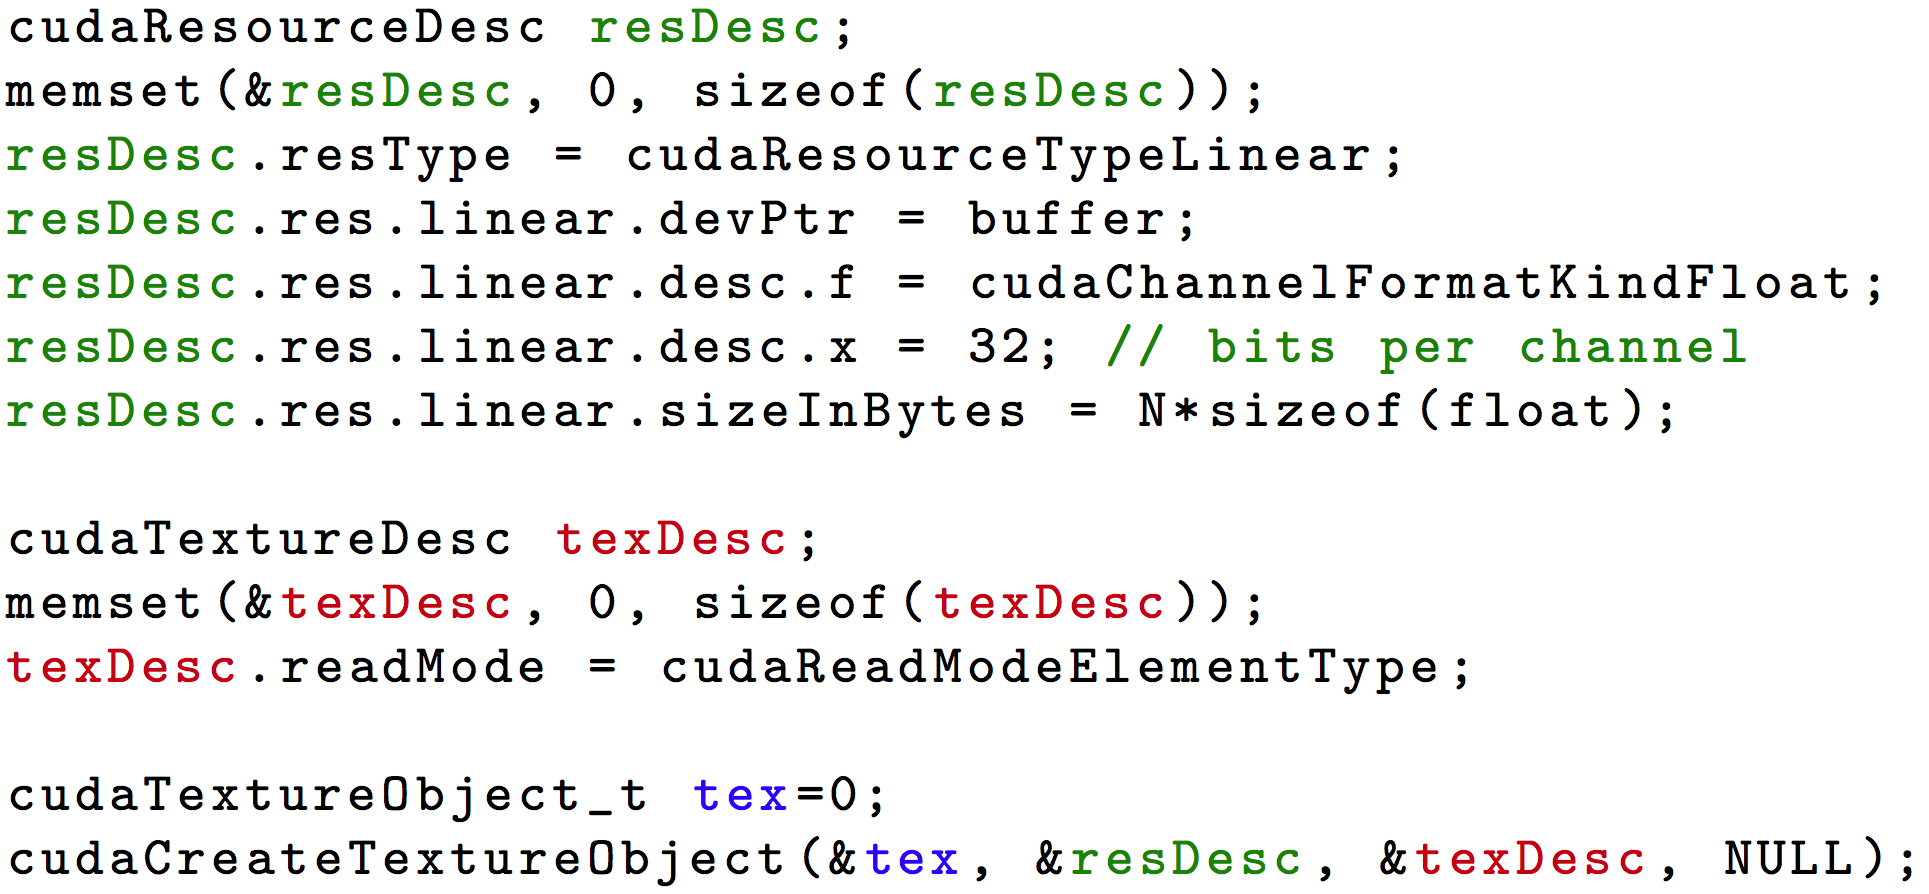
\includegraphics[width=0.80\textwidth]{figures/CudaTextureCode}

  \vspace{0pt}
  \pause
  \textbf{Kokkos} can hide mechanisms like that as simple as:
  \vspace{-5pt}

  \begin{code}[keywords={}]
View< @boldconst@bold double***, Layout, Space,
     @boldMemoryTraits<RandomAccess> @bold> name(...);
  \end{code}

\end{frame}

%==========================================================================

\begin{frame}[fragile]{Scatter Contribute (1)}

  Histogram generation is an example of the \textbf{Scatter Contribute} pattern.
 
  \begin{itemize}
    \item{Like a reduction but with many results.}
    \item{Number of results scales with number of inputs.}
    \item{Each results gets contributions from a small number of inputs/iterations.}
    \item{Uses an inputs-to-results map not inverse.}
  \end{itemize}

  \textbf{Examples:}
  \begin{itemize}
    \item{Particles contributing to neighbors forces.}
    \item{Cells contributing forces to nodes.}
    \item{Computing histograms.}
    \item{Computing a density grid from point source contributions.}
  \end{itemize}

\end{frame}

\begin{frame}[fragile]{Scatter Contribute (2)}

  \textbf{Compute forces on particles via neighbor contributions}

  This kernel uses Newtons Third Law: Actio = Reactio
  \begin{code}[keywords={void,int,parallel_for,for,View}]
void compute_forces(View<real3*> x, View<real3*> f,
	            View<int**> neighs, Interaction force) {
  int N = x.extent(0);
  int num_neighs = neighs.extent(1);
  parallel_for("ForceCompute", N, KOKKOS_LAMBDA(int i) {
    for(int j=0; j<num_neighs; j++) {
      real3 df = force.compute(x(i),x(neighs(i,j)));
      f(i) += df;
      f(j) -= df;
    }
  });
}
  \end{code}

  \pause
  \textbf{This kernel has a race condition on \texttt{f} though!}

\end{frame}

\begin{frame}[fragile]{ScatterView (0)}

  There are two useful algorithms:.
 
  \begin{itemize}
	  \item{\textbf{Atomics:} thread-scalable but depends on atomic performance.}
	  \item{\textbf{Data Replication:} every thread owns a copy of the output, not thread-scalable but good for low ($<16$) threads count architectures.}
  \end{itemize}

  \pause
  \begin{block}{Important Capability: ScatterView}
	  ScatterView can transparently switch between \textbf{Atomic} and \textbf{Data Replication} based scatter algorithms.
  \end{block}
  \pause
 	
  \begin{itemize}
	  \item{Abstracts over scatter contribute algorithms.}
	  \item{Compile time choice with backend-specific defaults.}
          \item{Only limited number of operations are supported.}
	  \item{Part of Kokkos Containers (in Kokkos 3.2 still experimental).}
  \end{itemize}

\end{frame}


\begin{frame}[fragile]{ScatterView (1)}
\textbf{Creating a ScatterView:}

Usually a \texttt{ScatterView} wraps an existing \texttt{View}
\pause
\begin{itemize}
  \item Allows the \textbf{atomic} variant to work without extra allocation.
\end{itemize}
\pause
\begin{code}[keywords={void,ScatterView,View,int}]
void compute_forces(View<real3*> x, View<real3*> f, 
	            View<int**> neighs, Interaction force) {
Kokkos::Experimental::ScatterView<real3*> scatter_f(f);
...
\end{code}

\pause
\textbf{Accessing the \texttt{ScatterView}}

In the kernel obtain an atomic or thread-local accessor.

  \begin{code}[keywords={access,auto,for,int}]
parallel_for("ForceCompute", N, KOKKOS_LAMBDA(int i) {
  auto f_a = scatter_f.access();
  for(int j=0; j<num_neighs; j++) {
    real3 df = force.compute(x(i),x(neighs(i,j)));
    f_a(i) += df;
    f_a(j) -= df;
  }
});
  \end{code}

  \pause
	\textbf{Only the \texttt{+=} and \texttt{-=} operators are available!}
\end{frame}

\begin{frame}[fragile]{ScatterView (2)}
We are missing one step though:
\pause
\textbf{Contribute back to the original view.}

  \begin{code}[keywords={void,View,ScatterView,int,contribute}]
void compute_forces(View<real3*> x, View<real3*> f,
	            View<int**> neighs, Interaction force) {
  Kokkos::Experimental::ScatterView<real3*> scatter_f(f);
  parallel_for("ForceCompute", N, KOKKOS_LAMBDA(int i) {
    ...
  });
  Kokkos::Experimental::contribute(f,scatter_f);
  \end{code}
\pause
\begin{itemize}
	\item No-op when \texttt{scatter\_f} uses \textbf{atomic} access
	\item Combines thread-local arrays in case of data duplication
\end{itemize}

\pause
	\begin{block}{Important Point}
		Reuse ScatterView if possible: creating and destroying data duplicates is costly and should be avoided
	\end{block}
\end{frame}

\begin{frame}[fragile]{ScatterView (3)}
	When reusing a \texttt{ScatterView} the duplicates have to be reset.

\begin{code}[keywords={reset}]
scatter_f.reset();
\end{code}

\pause
\textbf{The complete picture:}

  \begin{code}[keywords={ScatterView,reset,access,contribute}]
void compute_forces(View<real3*> x, View<real3*> f,
                    ScatterView<real3*> scatter_f,
	            View<int**> neighs, Interaction force) {
  scatter_f.reset();
  int N = x.extent(0);
  int num_neighs = neighs.extent(1);
  parallel_for("ForceCompute", N, KOKKOS_LAMBDA(int i) {
    auto f_a = scatter_f.access();
    for(int j=0; j<num_neighs; j++) {
      real3 df = force.compute(x(i),x(neighs(i,j)));
      f_a(i) += df;
      f_a(j) -= df;
    }
  });
  Kokkos::Experimental::contribute(f,scatter_f);
}
  \end{code}	
\end{frame}


\begin{frame}[fragile]{ScatterView (4)}
\textbf{But I need something else than a Sum!}

\pause
\texttt{ScatterView} has more options including the reduction op.

\begin{code}[keywords={template,class}]
  template<class DataType, class Layout, class Space,
	   class Operation, int Duplication, int Contribution>
  class ScatterView;
\end{code}
	\begin{itemize}
		\item \texttt{DataType}, \texttt{Layout}, \texttt{Space}:  as in \texttt{Kokkos::View}
		\item \texttt{Operation}: \texttt{ScatterSum}, \texttt{ScatterProd}, \texttt{ScatterMin}, or \texttt{ScatterMax}.
		\item \texttt{Duplication}: Whether to duplicate values per thread.
		\item \texttt{Contribution}: Whether to use \textbf{atomics}.
	\end{itemize}

\end{frame}


\begin{frame}[fragile]{Exercise ScatterView}

  \begin{small}
  \begin{itemize}
  \item Location: \ExerciseDirectory{scatter\_view/Begin}
  \item Assignment: Convert scatter\_view\_loop to use \texttt{ScatterView}.
  \item Compile and run on both CPU and GPU
  \end{itemize}
  \end{small}

\begin{code}
  # Compile for CPU
  cmake -B build_openmp -DKokkos_ENABLE_OPENMP=ON
  cmake --build build_openmp
  # Run on CPU
  ./build_openmp/scatterview -S 26
  # Note the warnings, set appropriate environment variables
  # Compile for GPU
  cmake -B build_cuda -DKokkos_ENABLE_CUDA=ON
  cmake --build build_cuda
  # Run on GPU
  ./build_cuda/scatterview -S 26
\end{code}

  \begin{scriptsize}
  \begin{itemize}
  \item Compare performance on CPU of the three variants
  \item Compare performance on GPU of the two variants
  \item Vary problem size: first and second optional argument
  \end{itemize}
  \end{scriptsize}

\end{frame}
%==========================================================================

\begin{frame}{Section Summary}

  \begin{itemize}
    \item Atomics are the only thread-scalable solution to thread safety.
      \begin{itemize}
        \item Locks or data replication are \textbf{not portable or scalable}
      \end{itemize}
    \item Atomic performance \textbf{depends on ratio} of independent work and atomic operations.
      \begin{itemize}
        \item With more work, there is a lower performance penalty, because of increased opportunity to interleave work and atomic.
      \end{itemize}
    \item The \texttt{Atomic} \textbf{memory trait} can be used to make all accesses to a view atomic.
    \item The cost of atomics can be negligible:
      \begin{itemize}
        \item \textbf{CPU} ideal: contiguous access, integer types
        \item \textbf{GPU} ideal: scattered access, 32-bit types
      \end{itemize}
    \item Many programs with the \textbf{scatter-add} pattern can be thread-scalably parallelized using atomics without much modification.
    %\item{Scatter-atomic-add \emph{can} have \textbf{negligible} cost for low contention ($< \sim100$) and non-trivial work.}
  \end{itemize}

\end{frame}

%==========================================================================

\begin{frame}[fragile]{DualView}

  {\Huge DualView}

  \vspace{20pt}

  \textbf{Learning objectives:}
  \begin{itemize}
    \item{Motivation and Value Added.}
    \item{Usage.}
    \item{Exercises.}
  \end{itemize}

\end{frame}

%==========================================================================

\begin{frame}[fragile]{DualView(0)}

  \textbf{Motivation and Value-added}

  \vspace{1em}

  \begin{itemize}
  \item{DualView was designed to help transition codes to Kokkos.}
  \pause
  \vspace{10pt}
  \item{DualView simplifies the task of managing data movement between memory spaces, e.g., host and device.}

  \pause
  \vspace{10pt}
  \item{When converting a typical app to use Kokkos, there is usually no holistic view of such data transfers.}
  \end{itemize}


\end{frame}
%==========================================================================

\begin{frame}[fragile]{DualView(1)}
\begin{figure}[h]
  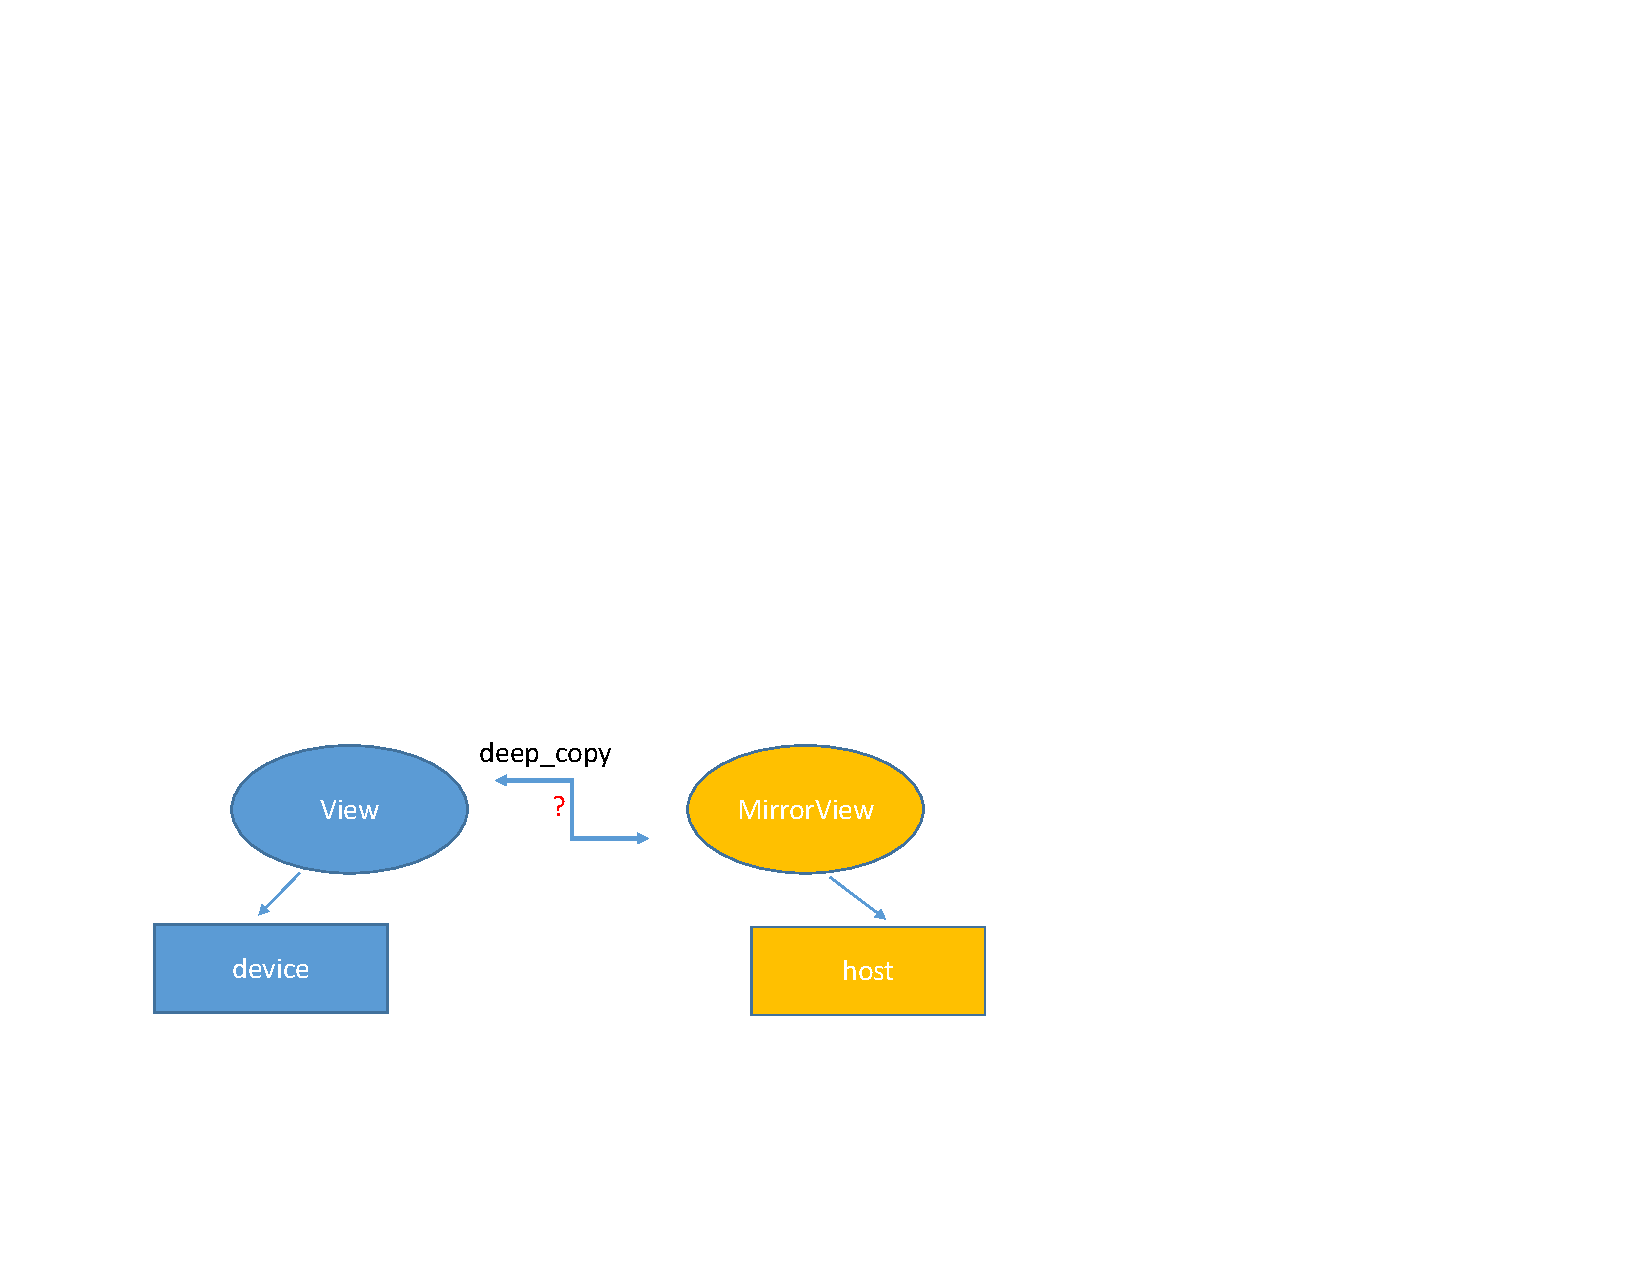
\includegraphics[height=1in]{figures/DualView_hostMirror.pdf}
\end{figure}

\textbf{Without DualView, could use MirrorViews, but}
  \begin{itemize}
    \item{deep copies are expensive, use sparingly}
    \item{do I need a deep copy here?}
    \item{where is the most recent data?}
    \item{is data on the host or device stale?}
    \item{was code modified upstream? is data here now stale, but not in previous version?}
  \end{itemize}

\end{frame}


%==========================================================================

\begin{frame}[fragile]{DualView: Usage}

\vspace{1em}
  \textbf{DualView bundles two views, a Host View and a Device View}

\begin{figure}[h]
 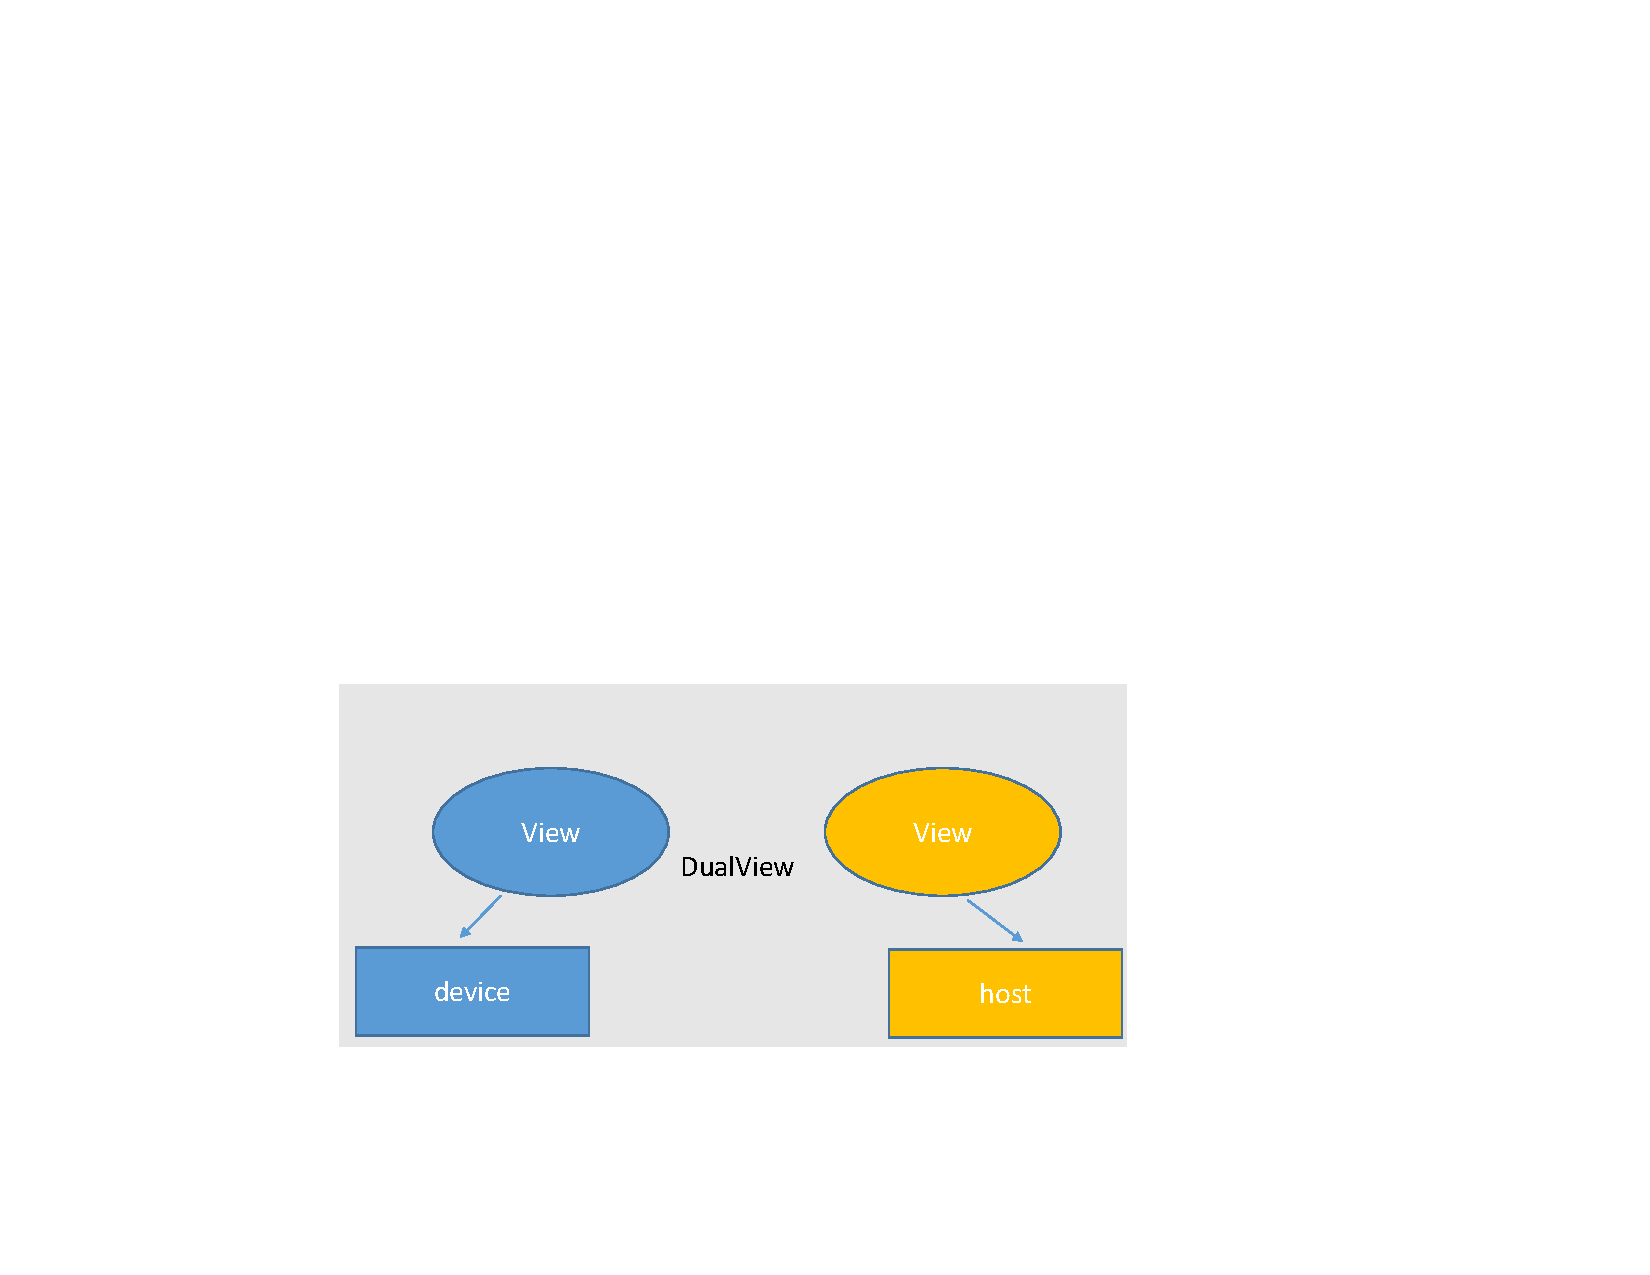
\includegraphics[height=1.25in]{figures/DualView_dualView.pdf}
\end{figure}

\textbf{There is no automatic tracking of data freshness:}
\begin{itemize}
\item  you must tell Kokkos when data has been modified on a memory space.
\item If you mark data as modified when you modify it, then Kokkos will know if it needs to move data
\end{itemize}
\end{frame}

%==========================================================================

\begin{frame}[fragile]{DualView: Usage(1)}
\vspace{1em}
  \textbf{DualView bundles two views, a Host View and a Device View}
  \begin{itemize}
    \item{Data members for the two views}
      \begin{code}[frame=single, keywords={}]
          DualView::t_host h_view
          DualView::t_dev  d_view
       \end{code}
    \item{Retrieve data members}
      \begin{code}[frame=single, keywords={}]
          t_host view_host();
          t_dev  view_device();
      \end{code}
    \item{Mark data as modified}
      \begin{code}[frame=single, keywords={}]
          void modify_host();
          void modify_device();
      \end{code}
  \end{itemize}
\end{frame}

\begin{frame}[fragile]{DualView: Usage(2)}
\vspace{1em}
  \textbf{DualView bundles two views, a Host View and a Device View}
  \begin{itemize}
    \item{Sync data in a direction if not in sync}
      \begin{code}[frame=single, keywords={}]
          void sync_host();
          void sync_device();
      \end{code}
    \item{Check sync status}
      \begin{code}[frame=single, keywords={}]
          bool need_sync_host();
          bool need_sync_device();
      \end{code}
   \end{itemize}
\end{frame}

\begin{frame}[fragile]{DualView: Usage in generic context}
\textbf{DualView has templated functions for generic use in templated code}

  \begin{itemize}
    \item{Retrieve data members}
      \begin{code}[frame=single, keywords={}]
          template<class Space>
          auto view();
      \end{code}
\vspace{-0.2em}
    \item{Mark data as modified}
      \begin{code}[frame=single, keywords={}]
          template<class Space>
          void modify();
      \end{code}
\vspace{-0.2em}
    \item{Sync data in a direction if not in sync}
      \begin{code}[frame=single, keywords={}]
          template<class Space>
          void sync();
      \end{code}
\vspace{-0.2em}
    \item{Check sync status}
      \begin{code}[frame=single, keywords={}]
          template<class Space>
          bool need_sync();
      \end{code}
   \end{itemize}   
\end{frame}

\begin{frame}[fragile]{DualView Example}

\begin{code}[keywords={sync_device,modify_device,view_device,view_host,sync_host,modify_host,DualView}]
class Foo {
DualView<...> data;
void run_a() {
  data.sync_device(); data.modify_device();
  auto d_data = data.view_device();
  parallel_for(N, KOKKOS_LAMBDA(int i) { d_data(i)+=/*mod d_d*/});
}
void run_b() {
  data.sync_host(); 
  auto h_data = data.view_host();
  for(int i=0; i<N; i++) { h_data(i) += /* modify h_data */ });
  data.modify_host();
}
void run_c() {
  data.sync_device();
  auto d_data = data.view_device();
  parallel_for(N, KOKKOS_LAMBDA(int i) { /* read d_data */ });
}
void do_operations(bool a, bool b, bool c) {
  if(a) run_a();
  if(b) run_b();
  if(c) run_c();
}
};
\end{code}
\end{frame}
%==========================================================================

\begin{frame}[fragile]{Exercise - DualView}

  \textbf{Details}:
  \begin{small}
  \begin{itemize}
    \item Location: \ExerciseDirectory{dualview/Begin}
    \item Modify or create a new compute\_enthalpy function in dual\_view\_exercise.cpp to:
    \begin{itemize}
      \item 1. Take (dual)views as arguments
      \item 2. Call \textbf{modify()} and/or \textbf{sync()} when appropriate for the dual views
      \item 3. Runs the kernel on host or device execution spaces
    \end{itemize}
  \end{itemize}
  \end{small}

\begin{code}
  # Compile for CPU
  cmake -B build_openmp -DKokkos_ENABLE_OPENMP=ON
  cmake --build build_openmp
  # Run on CPU
  ./build_openmp/dualview
  # Note the warnings, set appropriate environment variables
  # Compile for GPU
  cmake -B build_cuda -DKokkos_ENABLE_CUDA=ON
  cmake --build build_cuda
  # Run on GPU
  ./build_cuda/dualview
\end{code}

\end{frame}

%==========================================================================


\begin{frame}[fragile]{Module 3: Summary}

	\textbf{MDRangePolicy}
        \begin{itemize}
                \item Tightly nested loops (similar to OpenMP collapse clause)
                \item Available with \texttt{parallel\_for} and \texttt{parallel\_reduce}
                \item Tiling strategy over the iteration space
                \item Control iteration pattern at compile time
        \end{itemize}

\begin{code}[keywords={double,Iterate,Left,Right,int,MDRangePolicy,Rank}]
View<double**,LayoutLeft> A("A",N0,N1);
parallel_for("Label",
  MDRangePolicy<Rank<2,Iterate::Left,Iterate::Left>>(
	{0,0},{N0,N1}),
  KOKKOS_LAMBDA(int i, int j) {
    A(i,j) = 1000.0 * i + 1.0*j;
});
\end{code}

\end{frame}

\begin{frame}[fragile]{Module 3: Summary}

	\textbf{Subviews}
        \begin{itemize}
                \item Taking slices of Views
                \item Similar capability as provided by Matlab, Fortran, or Python
                \item {Prefer the use of \texttt{auto} for the type
\begin{code}[keywords={View,int,subview,ALL,make_pair}]
View<int ***> v("v", N0, N1, N2);
auto sv = subview(v, i0, ALL, make_pair(start,end));
\end{code}}
        \end{itemize}

        \vspace{10pt}
        \textbf{Unmanaged Views}
        \begin{itemize}
                \item Interoperability with externally allocated arrays
                \item No reference counting, memory not deallocated at destruction
                \item { User is responsible for insuring proper dynamic and/or static extents, MemorySpace, Layout, etc.
\begin{code}[keywords={View, float, LayoutRight, HostSpace, MemoryTraits, Unmanaged}]
View<float**, LayoutRight, HostSpace>
  v_unmanaged(raw_ptr, N0, N1);
\end{code}}
        \end{itemize}

\end{frame}

\begin{frame}[fragile]{Module 3: Summary}

	\textbf{Atomic operations}
        \begin{itemize}
                \item Atomic functions available on the host or the device (e.g. \texttt{Kokkos::atomic\_add})
                \item {Use \texttt{Atomic} memory trait for atomic accesses on Views
\begin{code}[keywords={View,int,MemoryTraits,Atomic}]
View<int*> v("v", N0);
View<int*, MemoryTraits<Atomic>> v_atomic = v;
\end{code}}
                \item Use \texttt{ScatterView} for scatter-add parallel pattern
        \end{itemize}

        \vspace{10pt}
	\textbf{Dual Views}
        \begin{itemize}
                \item For managing data synchronization between host and device
 		\item Helps in codes with no holistic view of data flow
		\begin{itemize}
                   \item In particular when porting codes incrementally
                \end{itemize}
        \end{itemize}

\end{frame}
\begin{frame}{Module 4: Hierarchical Parallelism (08/07)}

	\vspace{5pt}
	\textbf{Hierarchical Parallelism}
	\begin{itemize}
        \item How to leverage more parallelism through nested loops.
        \item The concept of Thread-Teams and Vectorlength.
	\end{itemize}

	\vspace{5pt}
	\textbf{Scratch Space}
	\begin{itemize}
        \item Getting temporary workspace in kernels.
        \item Leveraging GPU Shared Memory.
	\end{itemize}

        \vspace{5pt}
        \textbf{Unique Token}
        \begin{itemize}
        \item How to acquire safely per-thread resources.
        \end{itemize}

	\vspace{10pt}
    \textbf{Slack channel:} {\scriptsize \url{https://kokkosteam.slack.com/}}
	
	\vspace{10pt}
	\textbf{Recordings/Slides:} {\scriptsize \url{https://kokkos.org/kokkos-core-wiki/videolectures.html}}

\end{frame}

\end{document}

